% !TEX root = ../thesis_main.tex
\chapter{Prior Ultrafast Spectroscopy Studies of SWCNTs}

\section{Introduction}

For bulk semiconductors and quantum well structures, it is understood that nonradiative carrier relxation processes can limit their use in the development of optoelectronic devices \cite{agrawal1986long, roulston1990bipolar, green1995silicon}. For instance, lasers require materials capable of achieving population inversion, a condition where a large density of electrons occupy an excited state that allows incident light to be amplified by stimulated emission \cite{agrawal1986long, siegman1986lasers}. However, processes such as Auger recombination, depicted in Figure \ref{fig:auger_recomb_meyaard}, can inhibit population inversion by allowing some electrons to relax back to the ground state in a nonradiative fashion. Here, one electron-hole pair can nonradiatively recombine whilst the excess energy is instead transferred to another electron which subsequently occupies a higher energy state \cite{beattie1959auger}.

\begin{figure}
	\centering
	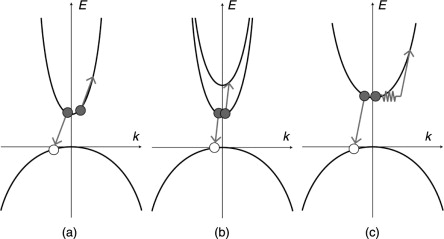
\includegraphics[trim = 0 0 3.2cm 0, clip]{images/chapter_prior_works/auger_schematic_meyaard}
	\caption{Schematic diagram of Auger recombination. In principle, Auger recombination can occur in the presence of 2 electrons and one hole. One electron-hole pair recombines in a nonradiative fashion and the remaining electron can access a higher energy state either (a) within the band it originally occupied or (b) within a higher energy subband. Reproduced and modified from \cite{meyaard2014efficiency}. }
	\label{fig:auger_recomb_meyaard}
\end{figure}

%Excitons are known to decay in a number of processes including electron-hole recombination which results in photon emission, or through other nonradiative processes such as phonon scattering or entrapment in defects or impurities \cite{simpson1957electronic}.
Excitons are also known to be capable of participating in a type of Auger recombination process known as exciton-exciton annihilation, which involves two excitons. One exciton nonradiatively recombines whilst the other gets promoted to a higher energy state. This was first explored conceptually by Northrop \textit{et al}.\ as a means of explaining the transport properties of molecular crystals \cite{northrop1958electronic}. Conventionally, exciton-exciton annihilation is modeled using the rate equation
%
\begin{equation}
	\frac{\partial n(\vec{r}, t)}{\partial t} = - \gamma n(\vec{r}, t)^2,
	\label{eq:rate_eq_exc_anih}
\end{equation}
%
where $n(\vec{r}, t)$ characterizes local exciton density at position $\vec{r}$ at time $t$ and $\gamma$ is a decay constant associated with exciton-exciton annihilation.

This phenomenon has also been explored in SWCNTs. However, there has been a substantial debate regarding the contribution of exciton-exciton annihilation in carrier dynamics of SWCNTs. Photoluminescence measurements suggest that exciton-exciton annihilation is a dominant carrier relaxation process that restricts the number of excitons that can be created. However, transient absorption experiments do not corroborate this observation. This apparent contradiction demonstrates a lack of consensus on the exact nature of the nonradiative phenomena occurring in SWCNTs.

Among the other optoelectronic applications, SWCNTs may also be useful for ultrafast, all-optical switching devices \cite{chai2017ultrafast}. Figure \ref{fig:optical_switch_chai_2017} shows a schematic diagram of how they work. These devices operate by using the photons from an optical pump to modulate, via a nonlinear optical process in a suitable medium, the transmission of probe photons that act as carriers of information \cite{chai2017ultrafast}. The optical Stark effect represents a nonlinear optical phenomenon that can be harnessed for such applications. In this phenomenon, the optical pump induces a nonlinear effect in the medium that coherently shifts the energy of an optical resonance detected by the probe photons.

\begin{figure}[ht]
	\centering
	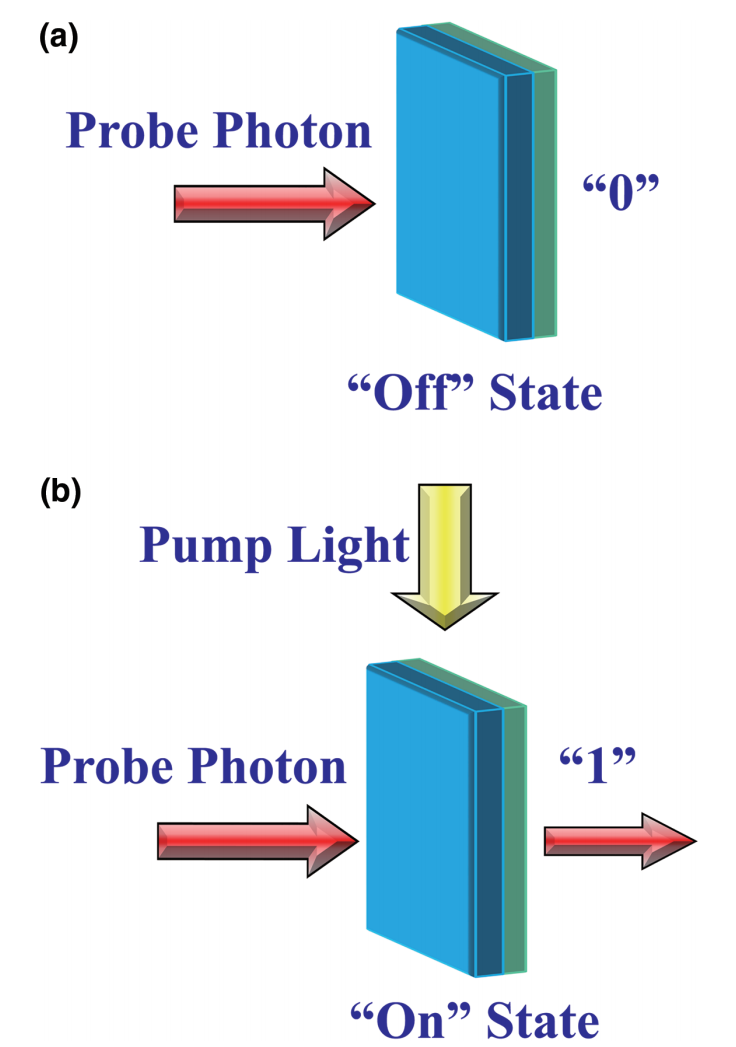
\includegraphics[scale=0.2]{images/chapter_prior_works/optical_switching_chai_2017}
	\caption{Schematic diagram showing the change in state of all-optical switching devices. (a) Without the presence of an optical pump, the state of probe photons incident on the nonlinear optical medium can be used as an OFF state (``0'') for device applications. (b) Incident photons from a sufficently intense optical pump will induce nonlinear optical phenomena in the medium. This effectively changes the state of the probe photons, and can be used as an ON (``1'') state. Reproduced from \cite{chai2017ultrafast}.}
	\label{fig:optical_switch_chai_2017}
\end{figure}

\section{Interband and Intersubband Recombination Dynamics}

Ostojic \textit{et al}.\ (2004) presented an early study regarding carrier relaxation and exciton recombination dynamics in carbon nanotubes \cite{ostojic2004interband}. They conducted wavelength-dependent, degenerate pump-probe measurements on an HiPco SWCNTs dispersed in an aqueous solution using sodium dodecyl sulfate (SDS) as a surfactant. %(See Sections \ref{section:cnt_synthesis} and \ref{section:dispersion_swcnt} for details).
Figure \ref{fig:abs_gordana} shows the optical absorption spectrum for their sample, which indicates the presence of many different chiralities, including both metallic and semiconducting nanotubes. The spectral region spanning $E_{1} H_{1}$ contains optical resonances associated with the $E_{11}$ transition occurring in semiconducting nanotubes. The region defined as $E_{2} H_{2}$ contains $E_{22}$ transitions of semiconducting nanotubes. Finally, the region labeled as Metallic exhibits the remaining $E_{11}$ resonances emerging from metallic nanotubes.

\begin{figure}[ht]
	\centering
	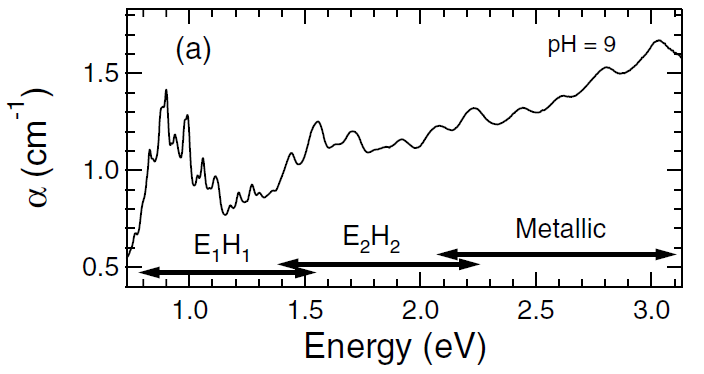
\includegraphics[scale=0.7]{images/chapter_prior_works/abs_gordana}

	\caption{Optical absorption spectrum for an aqueous suspension for HiPco SWCNTs individually suspended in an aqueous solution with sodium dodecyl sulfate (SDS) and studied by Ostojic \textit{et al}.\ (2004). The spectrum contains optical resonances associated with semiconducting nanotubes, which include $E_{11}$ in the region denoted as $E_{1} H_{1}$ as well as  $E_{22}$ in the region labeled as $E_{2} H_{2}$. The remaining resonances in the Metallic region come from the $E_{11}$ resonances of metallic nanotubes. Reproduced and modified from Ref.\ \cite{ostojic2004interband}.}
	\label{fig:abs_gordana}
\end{figure}

\begin{figure}[ht]
	\centering
	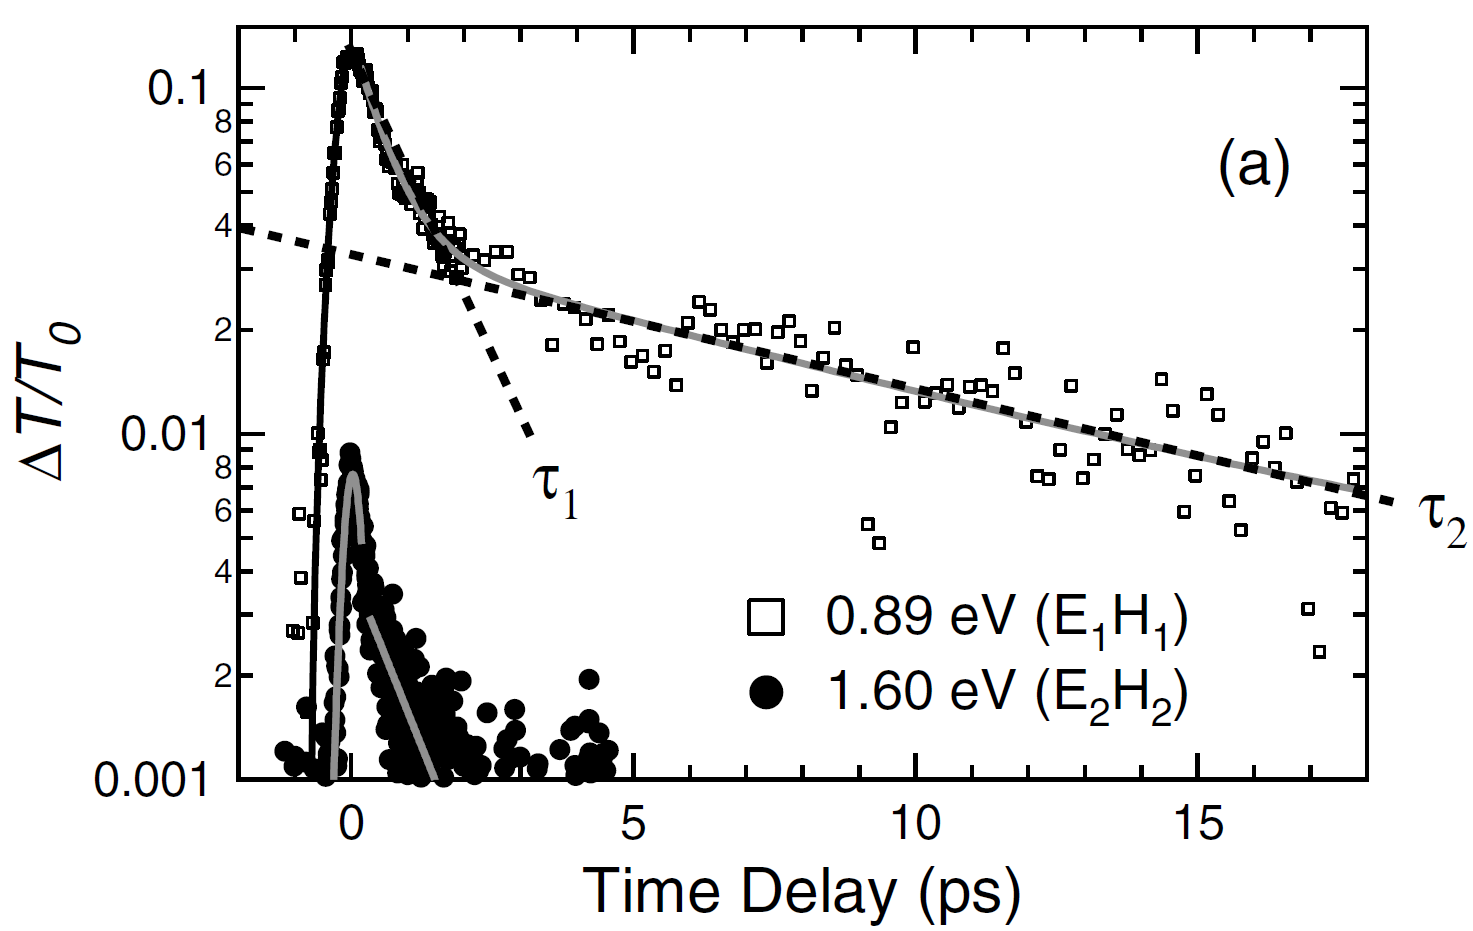
\includegraphics[scale=0.3]{images/chapter_prior_works/dtt_gordana}
	\caption{Differential transmission data at photon energies 0.89 eV (white squares) and at 1.60 eV (black circles) obtained from degenerate pump-probe measurements. At 1.60 eV, only a single fast exponential decay process associated with intraband relaxation is observed. At 0.89 eV, a bi-exponential decay occurs. The fast and slow components of the bi-exponential decay are associated with intraband and interband dynamics respectively. Reproduced and modified from Ref.\ \cite{ostojic2004interband}}
	\label{fig:dtt_gordana}
\end{figure}

The observed carrier dynamics showed a clear wavelength dependence as shown in Figure \ref{fig:dtt_gordana}. For pumping and probing within the $E_2 H_2$ region, the data was best described by a single exponential decay process, which was interpreted as intraband relaxation to lower-energy states. In contrast, a bi-exponential decay process was observed when pumping and probing in the $E_1 H_1$ region. The initial, fast decay was interpreted as intraband relaxation. However, the following slow exponential decay process was interpreted as interband relaxation. At the time of publication, this slow exponential decay process had not been observed before. Previous studies had only reported data obtained from nanotube bundles which exhibit significantly broader optical resonance that smear out the optical resonances of individual chiralities more so than in dispersions of individully suspended SWCNTs. \cite{ostojic2004interband}. In nanotube bundles, semiconducting nanotubes gain an additional nonradiative relaxation pathway via electrical contact with metallic nanotubes \cite{maeda2006gigantic}. However, in micelle-suspended samples these relaxation pathways through tube-tube contact no longer occur as surfacants prevent nanotubes from making physical contact.

\begin{figure}[ht]
	\centering
	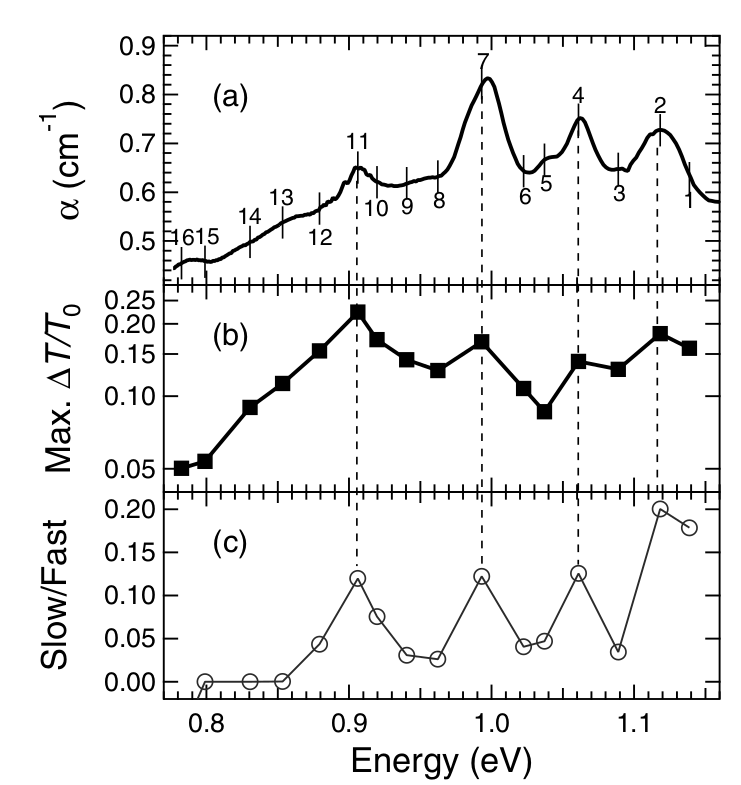
\includegraphics[scale=0.3]{images/chapter_prior_works/wavelength_dependence_gordana}
	\caption{(a) Optical absorption spectrum of HiPco SWCNTs individually suspended in an aqueous solution using sodium dodecyl sulfate (SDS) as a surfactant. The labeled positions indicate photon energies at which pump-probe measurements were taken. (b) Maximum differential transmission recorded at each measured photon energy. Differential transmission appears to reach a local maximum when the photon energy matches an optical resonance. (c) Ratio between the slow and fast decay times at each measured photon energy. The slow decay time reaches a local maximum when pumping at an optical resonance. Reproduced and modified from Ref.\ \cite{ostojic2004interband}}
	\label{fig:wl_dep_gordana}
\end{figure}

Ostojic \textit{et al}.\  also noted that for any chosen wavelength in their degenerate pump-probe study, some nanotubes are resonantly excited whereas others are photoexcited in a nonresonant fashion. This can affect the observed carrier decay dynamics. Figure \ref{fig:wl_dep_gordana} demonstrates this behavior. When the sample is excited at an optical resonance, the ratio between the slow and fast decay times reaches a local maximum. In contrast, when the sample is pumped at photon energies that do not exhibit a well-defined resonance, this ratio diminishes.

Hence, resonant excitation enhances the appearance of interband recombination dynamics. However, nonresonant excitations are more associated with the fast intraband dynamics. This suggests that the reported decay times only yield statistical averages of the carrier lifetime of the ensemble of all nanotubes that have optical resonances at energies less than or equal to the pump photon energy. Furthermore, they acknowledged that they did not observe a clear correlation between the power of the optical pump and the observed carrier decay times. This excludes the observation of any nonlinear, nonradiative recombination mechanisms such as Auger recombination, also referred to as exciton-exciton annihilation in this context.

Decreasing the pH of the sample was observed to suppress optical absorption peaks, especially those occurring at lower photon energies, as shown in Figure \ref{fig:ph_abs_gordana}. Correspondingly, the presence of the slow exponential decay process also diminished as shown in Figure \ref{fig:dtt_ph_gordana}. These effects were understood as a consequence of the Burstein-Moss effect, which is effectively the same as Pauli blocking. In other words, H$^+$ ions of the acidic aqueous suspension dope suspended SWCNTs by accepting negatively-charged carriers. This effect was most noticable at a pH of 4.5. Doping the individually suspended SWCNTs positions the Fermi level primarily within the valence band for nanotubes with larger diameters due to their smaller acceptor binding energies associated with their smaller effective masses.  As a result, the appearance of an interband absorption peak diminishes which subsequently removes the possibility of enhancing the occurrence of the interband relaxation by photoexciting at well-defined optical resonances.

\vspace{3cm}

\begin{figure}[H]
	\centering
	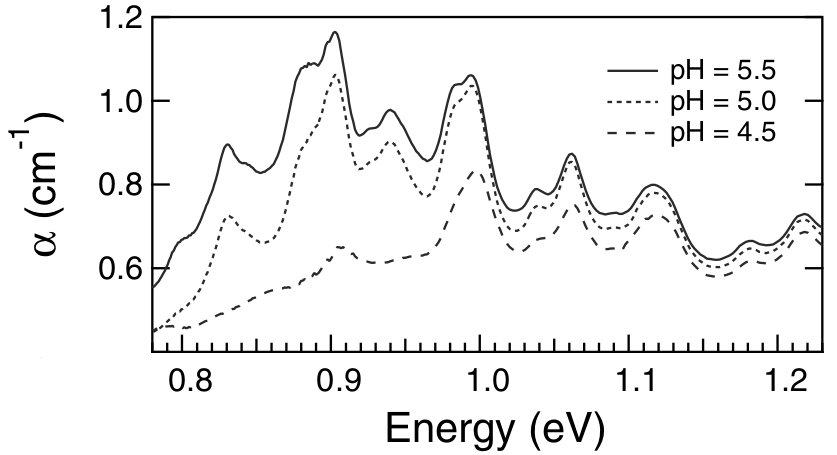
\includegraphics[scale=1.5]{images/chapter_prior_works/ph_effect_gordana_revised}
	\caption{The effect of pH on linear absorption. As the pH reduces from 5.5 to 4.5, absorption peaks at lower photon energies become supressed. This occurs as a consequence of the Burstein-Moss effect, as H$^+$ ions act as dopants that accept electrons. These dopants primarily affect larger-diameter nanotubes, as they exhibit lower binding energies for acceptors in light of their smaller effective masses. Reproduced and modified from Ref.\ \cite{ostojic2004interband}.}
	\label{fig:ph_abs_gordana}
\end{figure}

\begin{figure}[H]
	\centering
	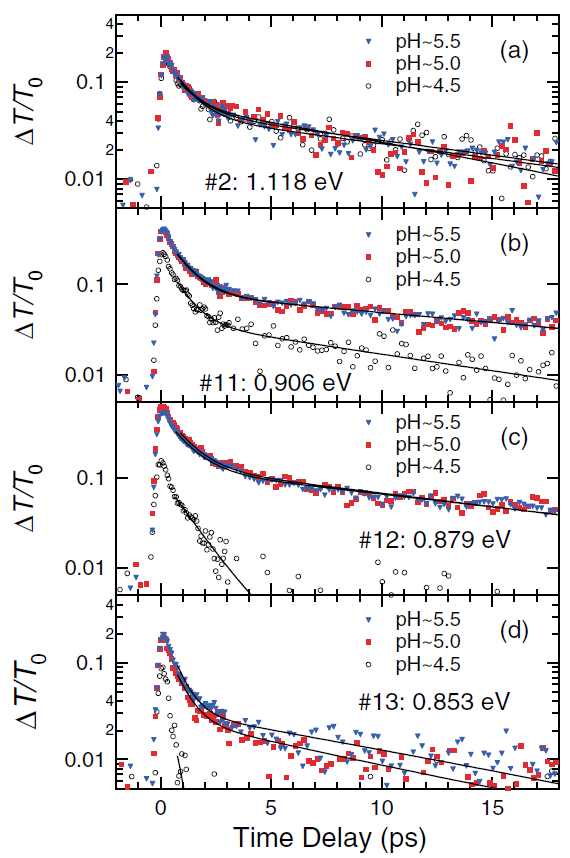
\includegraphics[scale=0.5]{images/chapter_prior_works/dtt_ph_gordana}
	\caption{The effect of pH on the carrier dynamics of nanotubes. Each plot corresponds to a degenerate pump-probe experiment conducted at a specified photon energy. As pH decreases, nanotubes become increasingly doped with positively-charge carriers. This has a larger effect on larger-diameter nanotubes due to their lower acceptor binding energies and lower the Fermi level into the valence band. At lower photon energies, the interband recombination process does not appear as the optical resonances associated with this process become supressed due to Pauli blocking, commonly referred to as the Burstein-Moss effect in this context. Reproduced and modified from Ref.\ \cite{ostojic2004interband}}
	\label{fig:dtt_ph_gordana}
\end{figure}

One final interesting detail about this study is that Ostojic \textit{et al.} affirm that these pH-dependent effects were not observed when using other anionic surfactants instead of SDS. They explained that this may be due to surface chemistry related to the micelle structures that form on the surfaces of nanotubes suspended using such surfactants, which could have some influence on nonradiative recombination rates. Indeed, this sheds light on a possible explanation regarding other heavily debated aspects of carrier dynamics in SWCNTs, such as the dominance of exciton-exciton annihilation, that have yet to be resolved. These studies, which will be discussed further in the following pages, all used different types of surfactants to create individually suspended SWCNTs ensembles, which has led to some apparent inconsistencies in the observations of carrier dynamics in SWCNTs. Thus far, the full extent at which surfactants affect carrier dynamics in SWCNTs remains to be explored.

Manzoni \textit{et al.}\ (2005) investigated the intersubband dynamics of SWCNTs using nondegenerate pump-probe measurements with a time resolution of 40 fs \cite{manzoni2005intersubband}. The sample they studied was a nanotube film made using HiPCo SWCNTs that were individually suspended using poly(ethylene glycol). Figure \ref{fig:abs_manzoni} shows the optical absorption spectrum for this sample along with the specta of the pump pulses used in this study. The sample contained a variety of optical resonances that belong to semiconducting and metallic nanotubes. The spectral regions labeled as EX1, EX2, and EX3 indicate the $E_{11}$, $E_{22}$, and $E_{33}$ resonances of semiconducting nanotubes, respectively. The region marked as Metallic shows the $E_{11}$ resonances for metallic nanotubes.

\begin{figure}[H]
	\centering
	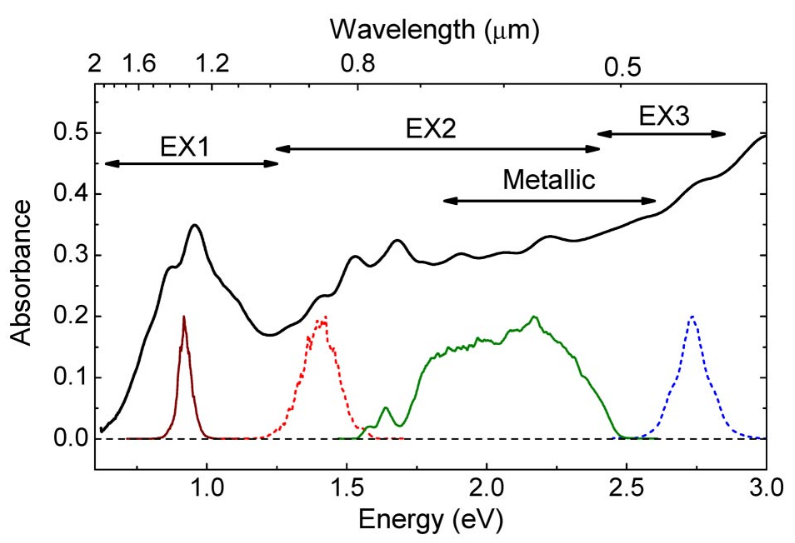
\includegraphics[scale=0.45]{images/chapter_prior_works/abs_manzoni}
	\caption{The black, solid line up top shows the absorption spectrum for a film of HiPco SWCNTs film individually suspended using poly(ethylene glycol) and studied by Manzoni \textit{et al}. (2005). The spectral regions indicated as EX1, EX2, and EX3 contain the $E_{11}$, $E_{22}$, and $E_{33}$ transitions of semiconducting nanotubes, respectively. The region labeled as Metallic contains the $E_{11}$ resonance of metallic nanotubes. The plots shown below represent the spectra of optical pump pulses used to photoexcite the SWCNT sample in this study. Reproduced and modified from Ref.\ \cite{manzoni2005intersubband}.}
	\label{fig:abs_manzoni}
\end{figure}

Depending on the pump and probe photon energies, the observed carrier relaxation dynamics exhibited either photoinduced transmission or photoinduced absorption. For instance, Figure \ref{fig:e11_pump_manzoni} shows the experimental results obtained when pumping in the EX1 region at 0.92 eV. The differential transmission signal probed at 0.95 eV shows clear signs of photobleaching, which indicates a finite population of photoexcited carriers. In contrast, the dynamics probed at 2 eV indicate the presence of photoinduced absorption.

\begin{figure}[H]
	\centering
	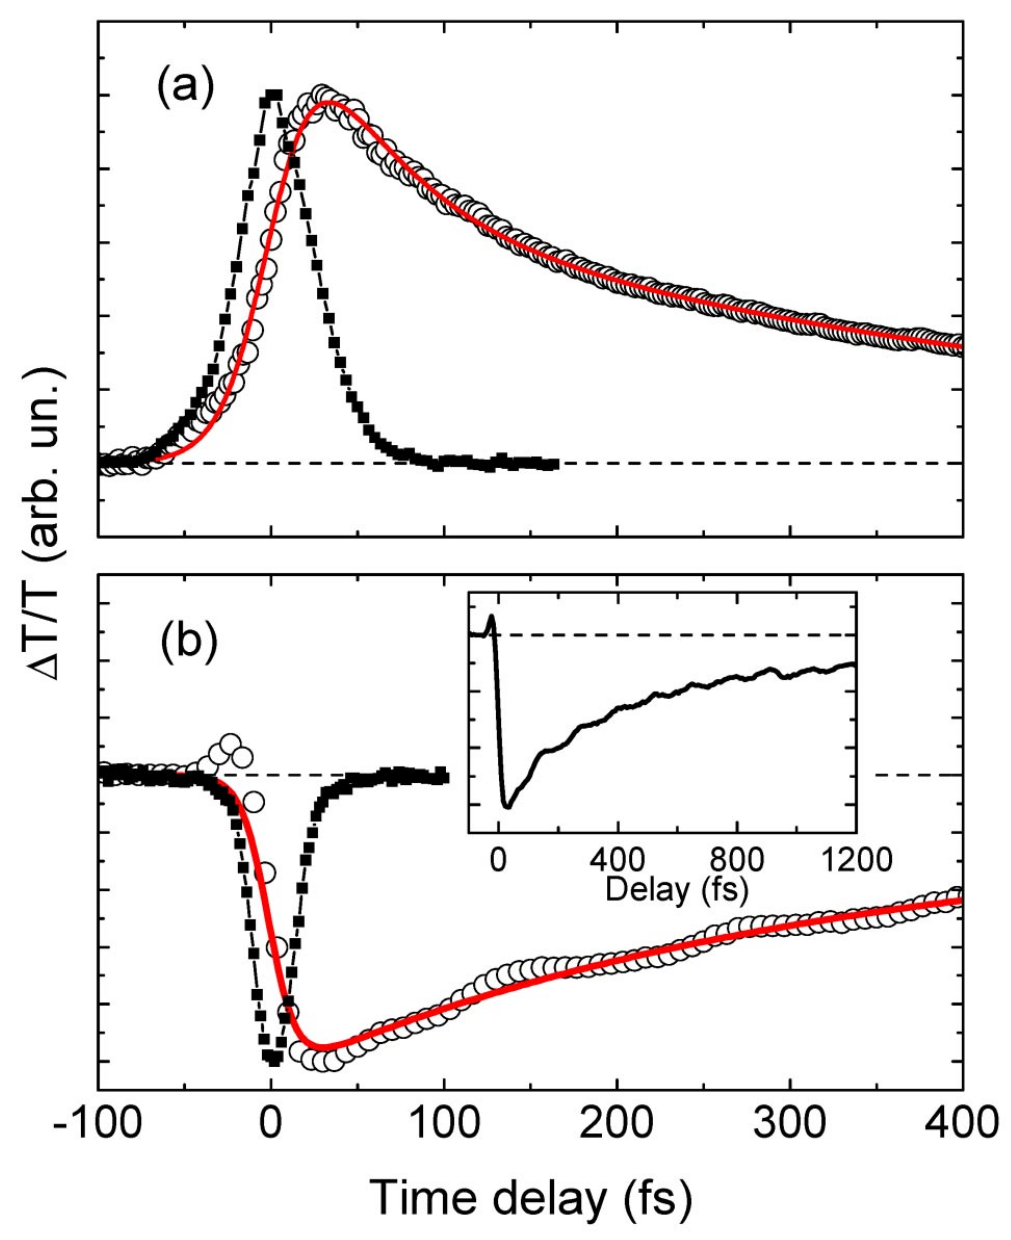
\includegraphics[scale=0.25]{images/chapter_prior_works/e11_pump_probe_manzoni}
	\caption{Carrier relaxation dynamics of SWCNTs photoexcited at 0.92 eV. Under this condition, the two plots correspond to differential transmission probed at 0.92 eV (a) and probed at 2.15 eV (b). The inset figure shows the relaxation measured at 2 eV on a longer time scale. The open circles represent the experimental data, and the solid lines indicate numerical fits to the data. The autocorrelation measurement of the pump pulse is also overlayed on both figures (squares + line). Reproduced from Ref.\ \cite{manzoni2005intersubband}.}
	\label{fig:e11_pump_manzoni}
\end{figure}

Photobleaching does not occur due to the fact that the photon energy of the pump is below the photon energies of the resonances in EX2. Hence, this photoinduced absorption was interpreted to occur due to an intersubband transition between a state in the EX1 region and another appropriate state located in EX3 as the energy difference between two such states would be on the order of 2 eV. Additionally, this probe signal at 2 eV exhibited an oscillatory component that was attributed to a radial breathing mode (RBM) of semiconducting CNTs that occurs at a frequency of 259~$\text{cm}^{-1}$. From examining Raman spectra, this indicated that SWCNTs such as (10,3), (11,1), (9,4) and (9,4) were photoexcited in this measurement.

When the SWCNTs were excited at an energy of 2.15 eV in the EX2 region, different dynamics occurred, as shown in Figure \ref{fig:e22_pump_manzoni}. Photobleaching occurred at the probed photon energy of 0.95 eV. In addition, both photoinduced transmission and absorption occurred at the probed photon energy of 2.15 eV. The initial photobleaching indicates a finite population of $E_{22}$ excitons. Furthermore, the decay occuring afterwards indicates the relaxation from $E_{22}$ to $E_{11}$. This process occurs on a time scale of 150 fs with an associated exponential decay constant of $\sim$40 fs. The photoinduced absorption was again interpreted to occur due to a possible transition between an EX1 state and an EX3. An oscillatory signal was also observed here, which was associated with an RBM frequency of 246 $\text{cm}^{-1}$ linked with nanotubes such as (10,3), (9,5), (9,4), and (7,6).

Figure \ref{fig:e33_pump_manzoni} illustrates the effect of photoexciting at 2.75 eV (EX3) and probing at 2.1 eV (EX2). Under these conditions, a small photobleaching signal followed by photosinduced absorption occurred. This demonstrated the fast relaxation dynamics from EX3 states into EX1 states. Furthermore, the time constant for this process was found to be $\sim$65 fs. Similar to the previous observations, the photoinduced absorption observed at EX2 indicated the carrier occupation of EX1 states.

\begin{figure}[H]
	\centering
	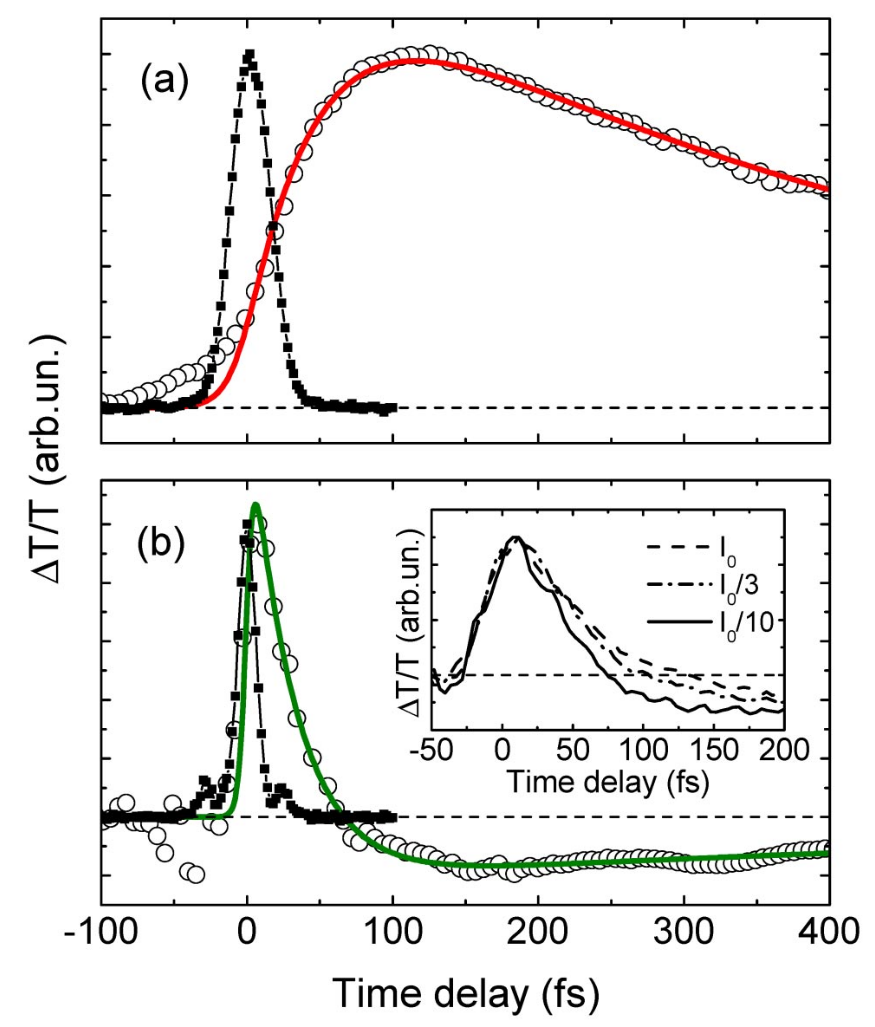
\includegraphics[scale=0.3]{images/chapter_prior_works/e22_pump_probe_manzoni}
	\caption{Differential transmission dynamics of a film of chirality-mixed HiPco SWCNTs photoexcited at 2.15 eV. Under this condition, the two plots correspond to differential transmission probed at 0.95 eV (a) and probed at 2 eV (b). The inset figure shows the pump power dependence measurements of the differential transmission probed at 2 eV. The open circles represent the experimental data, and the solid lines indicate numerical fits to the data. The autocorrelation measurement of the pump pulse is also overlayed on both figures (squares + line). Reproduced from Ref.\ \cite{manzoni2005intersubband}.}
	\label{fig:e22_pump_manzoni}
\end{figure}

Finally, Manzoni \textit{et al}.\ mentioned that they observed a weak relationship between optical pump intensity and observed recombination dynamics, as shown in the inset plot of Figure \ref{fig:e22_pump_manzoni}. At higher pump intensities, the time constant for the exponential decay did not change in a significant fashion. Thus, they did not observe exciton-exciton annihilation in their studies.

\begin{figure}[H]
	\centering
	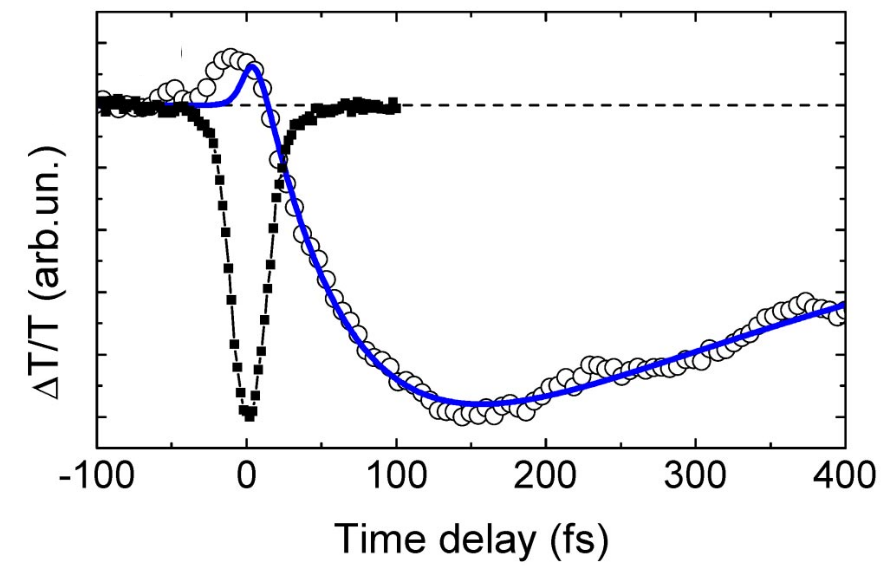
\includegraphics[scale=1.3]{images/chapter_prior_works/e33_pump_e22_probe_manzoni}
	\caption{Differential transmission dynamics of a film of chirality-mixed HiPco SWCNTs photoexcited at 2.75 eV and probed at 2.1 eV. The open circles represent the experimental data, and the solid line indicates a numerical fit to the data. The autocorrelation measurement of the pump pulse is also overlayed on the plot (squares + line). Reproduced from Ref.\ \cite{manzoni2005intersubband}.}
	\label{fig:e33_pump_manzoni}
\end{figure}


In general, excitons are expected to be stable in a scenario where their Bohr radius $r_\text{Bohr}$ is much smaller than the typical interexciton distance $d_\text{exc}$ \cite{mott1961transition}. Increasing the density of excitons can establish a condition where
\begin{equation}
r_\text{Bohr} \approx d_\text{exc},
\end{equation}
once the density is greater than or equal to a critical value known as the Mott density \cite{mott1961transition}. This causes a Mott transition process to occur where screening effects suppress the Coulomb interaction between electrons and holes, causing them to dissociate to create a free electron-hole plasma \cite{mott1961transition}. Ostojic \textit{et al}.\ (2005) investigated this phenomenon in SWCNTs using nondegenerate pump-probe spectroscopy, \cite{ostojic2005stability} featuring a broadband probe. They claimed that even at the Mott density, excitons still remain stable.

\begin{figure}[ht]
	\centering
	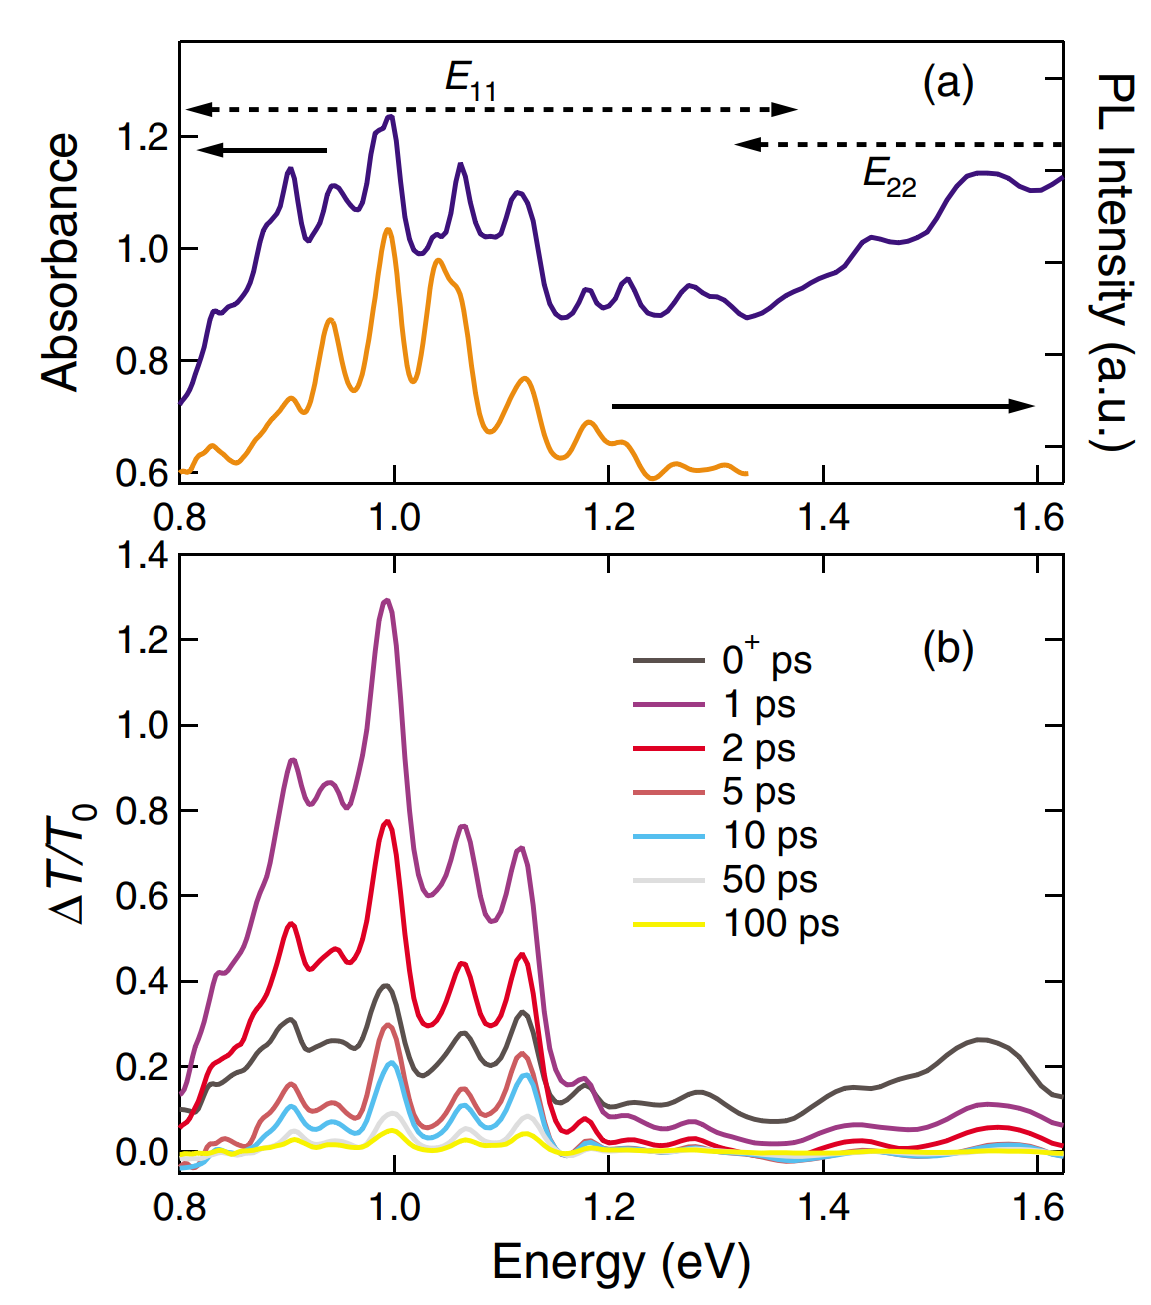
\includegraphics[scale=0.22]{images/chapter_prior_works/abs_dtt_gordana_2005}
	\caption{(a) Linear absorption (top curve, left axis) as well as photoluminescence spectra (bottom curve, right axis) of a  HiPco SWCNTs individually suspended in an aqueous solution using surfactants. (b) Differential transmission data taken at the given time delays after photoexciting at 1.60 eV. Reproduced from Ref.\ \cite{ostojic2005stability}. }
	\label{fig:abs_dtt_gordana_2005}
\end{figure}

Figure \ref{fig:abs_dtt_gordana_2005} shows the linear absorption and photoluminescence spectra for their sample containing HiPco SWCNTs that were micelle-suspended in heavy water (D$_2$O) as well as differential transmission spectra obtained at various time delays. The differential transmission data was taken using an optical pump centered at 1.6 eV. Within the first \SI{1}{\pico\second}, the signal observed within the $E_{22}$ range appears to decay, whereas that of the $E_{11}$ range increases rapidly. This agrees with the fast intersubband dynamics observed by Manzoni \textit{et al}.\ (2005) \cite{manzoni2005intersubband}. Moreover, the spectral shape of the differential transmisson stays constant and only changes in amplitude.


\begin{figure}[ht]
	\centering
	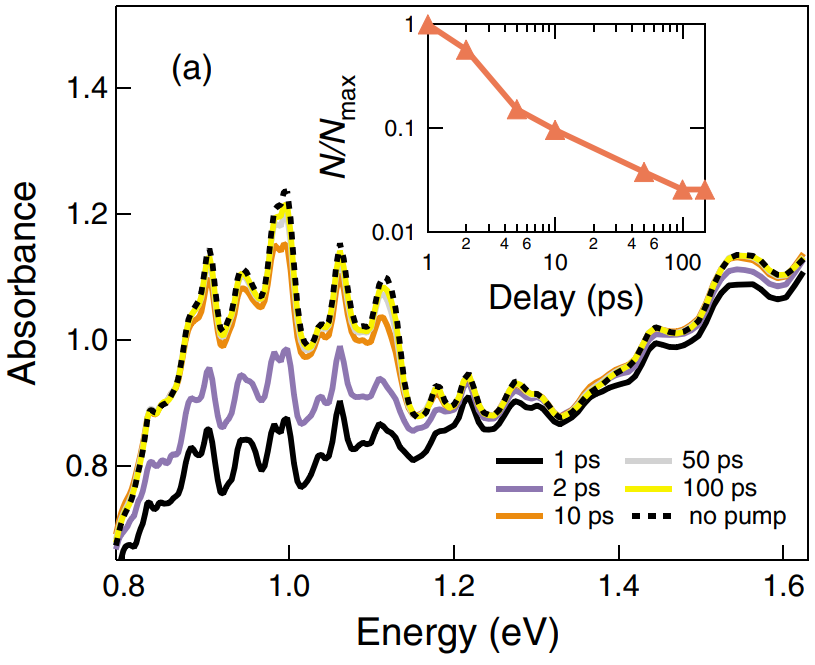
\includegraphics[scale=1.2]{images/chapter_prior_works/total_abs_gordana_2005}
	\caption{Total absorbance at each given time delay after accounting for the changes in transmission observed in Figure \ref{fig:abs_dtt_gordana_2005}(b). Despite the photobleaching that occurs, the exciton resonances do not change shape or undergo any shifts in energy. The inset figure shows how the normalized exciton density obtained by numerically integrating the differential absorbance varies with time. Reproduced from Ref.\ \cite{ostojic2005stability}.}
	\label{fig:total_abs_gordana_2005}
\end{figure}

These effects can be interpreted more easily by taking the linear absorption of the sample into account. Hence, Figure \ref{fig:total_abs_gordana_2005} shows how the total absorbance of the sample changes. The absorption associated with excitonic resonances decreases due to photobleaching effects. However, the overall shape of these resonances appears to remain constant. The peak positions do not shift in energy either.

Ostojic \textit{et al}.\ (2005) estimated the number of photoexcited excitons in nanotubes by taking into account the total number of nanotubes within the photoexcited volume of their sample, the change in absorbance, as well as the pump fluence \cite{ostojic2005stability}. They deduced that the density of excitons in a typical nanotube of length \SI{150}{\nm} is on the order of $5 \times 10^6$ \si{\per\cm}. This yields an average seperation of \SI{2}{\nm} between excitons. This result agreed with previous theoretical calculations in the literature suggested that the typical Bohr radius in SWCNTs of diameter 1 nm range between 2 - 5 \si{\nm} \cite{spataru2004excitonic, chang2004excitons}.

Estimates such as these imply that that shortly after photoexcitation, the optical pump creates enough excitons such that a Mott transition may indeed occur as the Bohr radius is of the same order of magnitude as the average interexciton distance. However, the presence that exciton resonances even at high pump fluences shows that excitons have not yet dissociated to form a free electron-hole plasma. Experimental results such as these have raised questions as to whether it is even possible to reach the Mott density in SWCNTs. Indeed, a number of studies have presented evidence that efficient exciton-exciton annihilation processes in SWCNTs establish an upper limit on the density of excitons that is below the Mott density.


\section{Exciton-Exciton Annihilation}

\subsection{Early Evidence in Support of Exciton-Exciton Annihilation}

Wang \textit{et al}.\ (2004) observed nonlinear recombination dynamics in time-resolve fluorescence experiments \cite{wang2004observation}. They performed these measurements on HiPco SWCNTs dispersed in an aqueous solution that were individually suspended using poly(acrylic acid). Figure \ref{fig:fluorescence_wang_2004} shows the key results of their study. At higher pump fluences, the onset of an early, fast exponential decay process becomes more prominent. This behavior exemplifies a well-known signature of Auger recombination processes. In addition, the fluorescence observed at longer time delays appears to saturate as shown in the inset plot of Figure \ref{fig:fluorescence_wang_2004}.

Furthermore, Figure \ref{fig:fast_slow_wang_2004} shows the time-integrated fluoresence contributions associated with the fast and slow decays. The fluorescence from the slow decay begins saturating at fluences greater than \SI{0.3}{\joule / \meter\squared}. In contrast, the time-integrated fluoresence linked with the fast decay only begins to saturate at a fluence of \SI{1.5}{\joule / \meter\squared}. These data suggest that exciton-exciton annihilation associated with the fast decay process establishes an upper limit of bright excitons that can exist at longer time delays.



Wang \textit{et al}.\ interpreted these results by devising a model of carrier dynamics that accounts for exciton-exciton annihilation processes. They postulate that the time-dependent probability density of a nanotube having $N$ electron-hole pairs $\rho^\text{N}(t)$ depends on the rate of radiate emission $\gamma^\text{N}_\text{r}$, the rate of exciton-exciton annihilation $\gamma^\text{N}_\text{A}$, as well as the rate of carrier trapping at defects $\gamma_\text{t}$. The master equation
\begin{equation}
	\dfrac{\mathrm{d}\rho^\text{N}}{\mathrm{d} t} = \rho^\text{N}(\gamma^\text{N+1}_\text{r} + \gamma^\text{N+1}_\text{A} + \gamma_\text{t})(N+1) - \rho^\text{N}(\gamma^\text{N}_\text{r} + \gamma^\text{N}_\text{A} + \gamma_\text{t})N,
\end{equation}
captures the relationship between these quantities.


In the case of excitons,
\begin{equation}
	\gamma^\text{N}_\text{r} = \text{const}, \text{   } \gamma^\text{N}_\text{A} = C_\text{A}(N-1),
\end{equation}
where $C_\text{A}$ is the exciton-exciton annihilation rate coefficient. This assumes that excitons radiatively recombine at a constant rate and that exciton-exciton annihilation rate for $N$ excitons is given as $C_\text{A}N(N-1)$. Radiative recombination scales linearly with $N$, whereas exciton-exciton annihilation scales as $N^2$ as expected. Moreover, the initial population of excitons is given as $N_\text{initial} = \phi \sigma$, where $\phi$ and $\sigma$ denote, respectively, the fluence of the optical pump and the absorption cross-section of carbon nanotubes.


Indeed, the quantitative results from this model agree with the experimental data presented in Figures \ref{fig:fluorescence_wang_2004} and \ref{fig:fast_slow_wang_2004}. Numerical fits to the data yield an estimate of $C_\text{A}$, which was found to be $\SI{0.8}{\per\pico\second}$. Correspondingly, this also provides an estimate of the typical lifetime of excitons that participate in exciton-exciton annihilation given as $1/\gamma^\text{N}_\text{A}$ which was determined to be on the order of picoseconds with lifetimes being as short as \SI{1.2}{\pico \second}.

\begin{figure}[H]
	\centering
	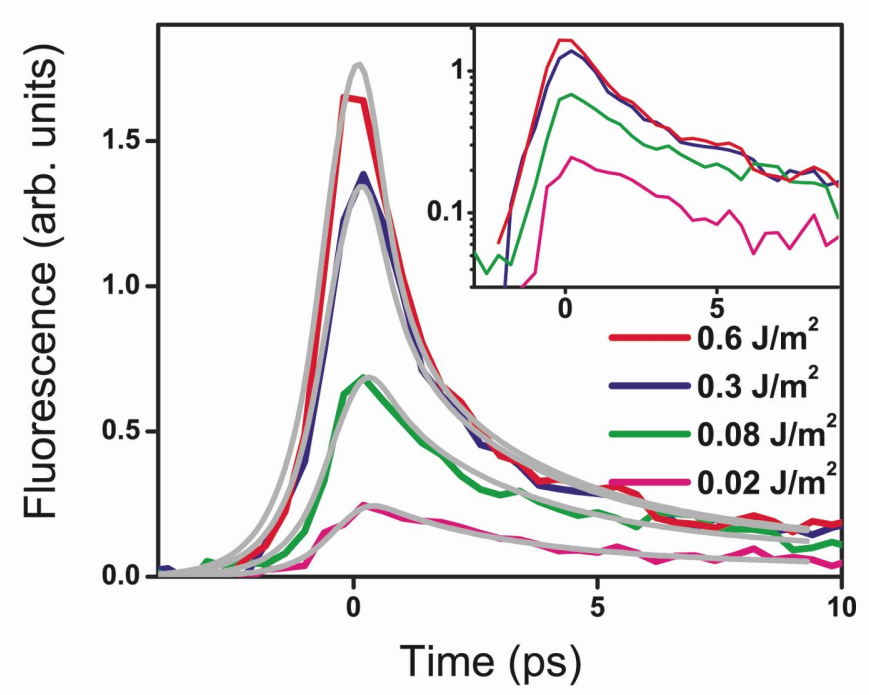
\includegraphics[scale=0.25]{images/chapter_prior_works/fluorescence_wang_2004}
	\caption{Time-resolved fluorescence captured from a micellar suspension of chirality-mixed HiPco SWCNTs dispersed in water using polyacrylic acid as a surfactant at indicated fluences. The optical pump pulse was centered 1.53 eV (810 nm). Gray curves are fits to the experimental data using a model based on exciton-exciton annihilation. At higher fluences, the dynamics exhibit a bi-exponential decay containing a fast and a slow process. The fast exponential decay has been attributed to the presence of a nonradiative decay mechanism associated with exciton-exciton annihilation, whereas the slow component emerges due to radiative interband recombination. The inset figure shows the same experimental data on a log-linear plot to emphasize the saturation of the fluoresence at higher pump fluences occuring due to nonradiative decay phenomena. Reproduced from Ref.\ \cite{wang2004observation}.}
	\label{fig:fluorescence_wang_2004}
\end{figure}


\begin{figure}[H]
	\centering
	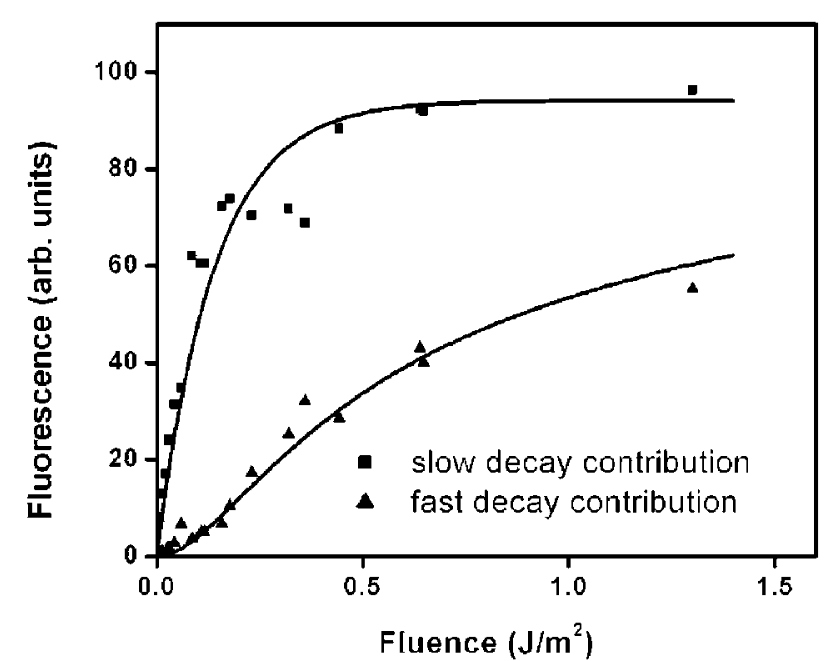
\includegraphics[scale=0.3]{images/chapter_prior_works/fast_slow_wang_2004}
	\caption{Time-integrated fluorscence associated with fast and slow decay contributions as a function of pump fluence. The solid curves represent fits to the data. The fluorescence associated with the slow decay saturates at a fluence above \SI{0.3}{\joule / \meter \squared}, indicating an upper limit of bright excitons. However, the time-integrated fluorescence of the fast decay only begins to saturate at \SI{1.5}{\joule / \meter \squared}. Reproduced from Ref.\ \cite{wang2004observation}.}
	\label{fig:fast_slow_wang_2004}
\end{figure}



Ma \textit{et al}.\ (2004) \cite{ma2004ultrafast} also obtained some experimental results that qualtitatively agree with those observed by Wang \textit{et al}.\ (2004) \cite{wang2004observation}. In this study, they performed both time-resolved fluorescence and time-resolved transient absorption measurements on a HiPco SWCNTs suspended in an aqueous solution using SDS. Figure \ref{fig:fluorescence_ma_2004} shows the fluorescence of (9,5) nanotubes that occurred after the sample was resonantly photoexcited at the $E_{22}$ energy. As the intensity of the optical pump increased, the presence of an early fast decay processes became more prominent close to time zero.

Here, Ma \textit{et al}.\ \cite{ma2004ultrafast} used the rate equation
\begin{equation}
	\dfrac{\mathrm{d}N(t)}{\mathrm{d}t} = - k N(t) - \gamma N(t)^2,
\end{equation}
to characterize the observed carrier dynamics. Here, $N$ denotes the average number of excitons at the $E_{11}$ energy level. The constants $k$ and $\gamma$ refer to the linear exciton decay rate and the exciton-exciton annihilation rate, respectively. If $kt < 1$, this gives the analytical solution
\begin{equation}
	N(t) = \dfrac{N(0)}{1 + N(0)\gamma \cdot t},
\end{equation}
where $N(0)$, a fitting parameter, yields the initial population of excitons.

\begin{figure}[H]
	\centering
	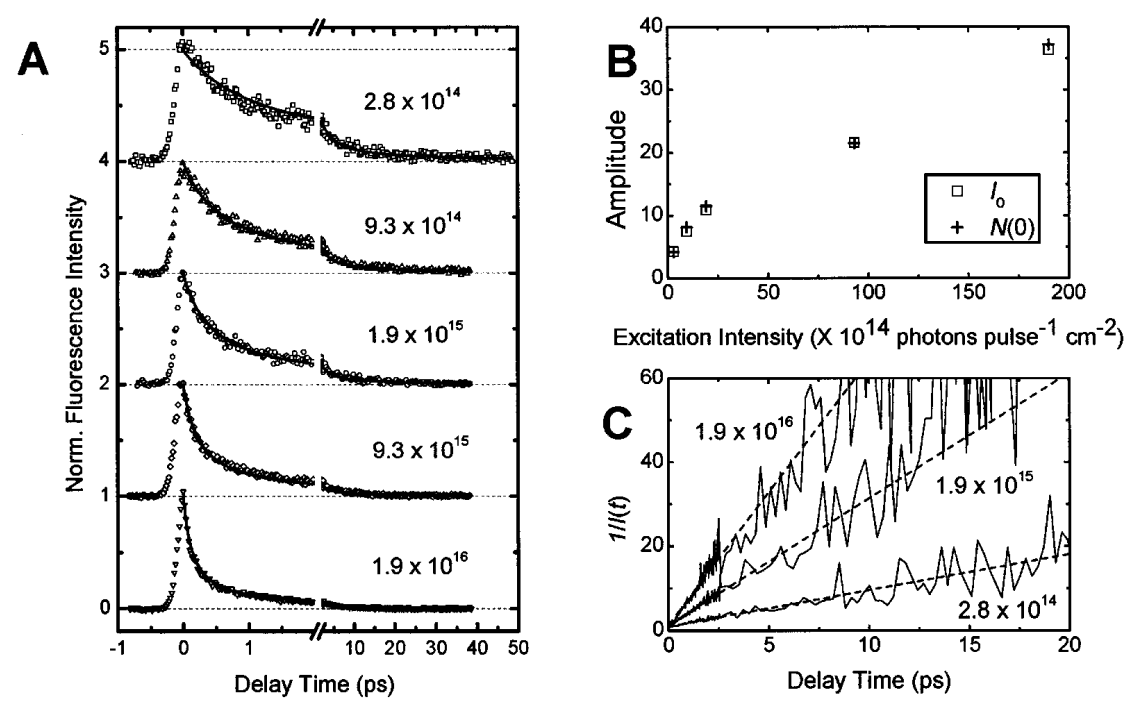
\includegraphics[scale=0.35]{images/chapter_prior_works/fluorescence_2_ma_2004}
	\caption{(a) Normalized time-resolved fluorescence measurements obtained from (9,5) nanotubes after exciting the $E_{22}$ resonance at different excitation fluences (photons\si{/\cm \squared}). At higher fluences, a fast decay component becomes more prominent. Solid lines represent fits to the data. (b) The maximum fluoresence intensity $I_0$ measured at each excitation fluence, along with the fitted parameter $N$(0). (c) The reciprocal of the fluorescence intensity taken at the labeled fluences and plotted as a function of time. The dashed lines represent fits to the data. Reproduced and modified from Ref.\ \cite{ma2004ultrafast}.}
	\label{fig:fluorescence_ma_2004}
\end{figure}

Furthermore, the assumption that the time-dependent, fluorescence intensity $I(t)$ is proportional to $ N(t)$ gives the expression
\begin{equation}
  	\left( \dfrac{I(t)}{I_0} \right)^{-1} \approx \left( \dfrac{N(t)}{N_0} \right)^{-1} = \gamma N(0) \cdot t + 1.
\end{equation}
%The results obtained from transient absorption measurements appear to exhibit some key differences from those obtained in the fluorescence measurements.
This suggests that the reciprocal of $I(t)$ has a linear dependence on time $t$ which certainly shows good agreement with the data, as shown in Figure \ref{fig:fluorescence_ma_2004}(c) except at longer time delays for higher pump fluences.



Figure \ref{fig:fluorescence_abs_ma_2004} shows more fluorescence and transient absorption data obtained by selectively photoexciting and probing resonances of (6,5) and (7,5) nanotubes, respectively, in the same chirality-mixed micelle-suspended sample used for the measurements shown earlier. More specifically, Figure \ref{fig:fluorescence_abs_ma_2004}(a) shows the fluorescence data obtained for (6,5) nanotubes after these nanotubes were resonantly excited at the $E_{22}$ photon energy. The results qualitatively match those of Figure \ref{fig:fluorescence_ma_2004}(a). However, the transient absorption data taken from (6,5) and (7,5) nanotubes after resonantly exciting their $E_{22}$ resonances and probing the dynamics at their respective $E_{11}$ energies appears to show some different carrier dynamics.

For the case of (6,5) nanotubes, Ma \textit{et al}.\ observed that the transient absorption curves show a weaker dependence on the pump intensity at fluences less than $2 \times 10^{15}$ photons/cm$^2$ \cite{ma2004ultrafast}. This of course contrasts with the fluorescence data, which shows a substantial pump intensity dependence at all reported fluences. In addition, they also observe some key differences between the transient aborption data taken for (6,5) and (7,5) nanotubes. When the sample was probed the $E_{11}$ resonance of (6,5) nanotubes, the transient absorption exhibited an early decay that became faster at higher fluences. However, for (7,5) nanotubes, this early decay instead became \textit{slower} at higher excitation intensities.

\begin{figure}[H]
	\centering
	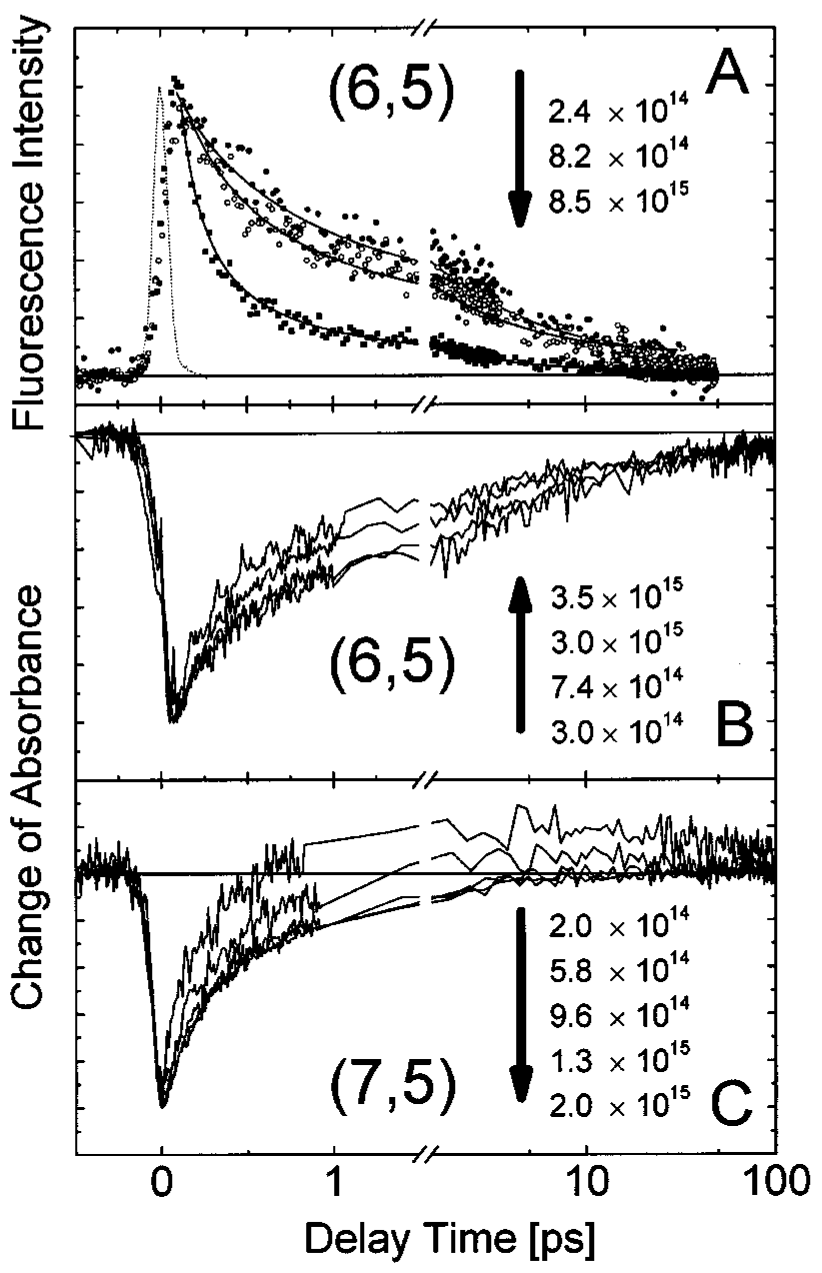
\includegraphics[scale=0.3]{images/chapter_prior_works/fluorescence_abs_2_ma_2004}
	\caption{(a) Time-resolved fluorescence measurements obtained for (6,5) nanotubes in a chirality-mixed SWCNT sample after resonantly exciting the $E_{22}$ state at the reported fluences (photons\si{/\cm \squared}). The dynamics show a clear dependence on intensity at all fluences. (b) Transient absorption data probed at the $E_{11}$ energy (6,5) carbon nanotubes after the sample was photoexcited at the $E_{22}$ resonance at the reported fluences. These show a weak pump intensity dependence at fluences below $2 \times 10^{15}$ photons/cm$^2$. The early decay also became faster at higher fluences. (c) Transient absorption data probed at the $E_{11}$ energy (7,5) carbon nanotubes after the sample was photoexcited at the $E_{22}$ resonance at the reported fluences. The early decay instead became much \textit{slower} at higher pump fluences. Reproduced from Ref.\ \cite{ma2004ultrafast}.}
	\label{fig:fluorescence_abs_ma_2004}
\end{figure}

These key differences lead Ma \textit{et al}.\ to conclude that a different set of carrier relaxation processes may be contributing to the transient absorption dynamics. In the case of (7,5) nanotubes, they interpreted that excitons may become trapped or even convert to triplet states. For (6,5) nanotubes, they suggested that the fluence threshold of $2 \times 10^{15}$ photons/cm$^2$ needed to observe clear nonlinear dynamics indicates that other than bright excitons, the probe may also be detecting the presence of unbound electron-hole pairs.



In a follow-up study, Ma \textit{et al}.\ (2005) measured transient absorption dynamics of (8,5) carbon nanotubes contained within an ensemble of HiPco SWCNTs dispersed in an aqueous solution using SDS as a surfactant \cite{ma2005femtosecond}. In this case, they attempted to account for the carrier dynamics occuring at both the $E_{11}$ and $E_{22}$ energy levels. Figure \ref{fig:exciton_schematic_ma} presents a schematic diagram of this approach. In this notation, each exciton band denoted as $E_i(\mathbf{k})$, where $\mathbf{k}$ represents the exciton center-of-mass momentum, contains $n_\text{i}$ excitons. Excitons at the lowest exciton band conduct exciton-exciton annihilation at rate $\gamma n_1^2/2$ which subsequently populates higher energy subbands. Finally, $k_\text{ij}$ represents linear relaxation rates from the $i$-th band to the $j$-th band, and $k_\text{1g}$ measures the relaxation rate from $E_i(\mathbf{k})$ to the ground state.


After assuming that the relaxation rates $k_\text{n2}$ and $k_\text{21}$ are very fast, which suggests that states other than those at $\mathbf{k} = 0$ are not occupied in this model, Ma \textit{et al}. deduced that
\begin{equation}
	n_2(t) \cong \frac{1}{2 k_{21}} \gamma n^2_1(t),
	\label{eq:ma_n2}
\end{equation}
where exciton-exciton annihilation in the $E_1(\mathbf{k})$ band quickly creates a population of excitons in the $E_2(\mathbf{k})$ band. Furthermore, they also stated that
\begin{equation}
\frac{\mathrm{d} n_1(t)}{\mathrm{d}t} = G(t) - \frac{1}{2}\gamma n_1^2(t) - k_\text{1g} n_1(t),
\end{equation}
where $G$($t$) represents the generation rate of excitons. This yields a formal solution that can be written as
%
\begin{equation}
	n_1(t) = \frac{n_1(0)e^{-k_\text{1g}t}}{1 + n_1(0) \gamma\cdot(1 - e^{-k_\text{1g}t} )/2k_\text{1g}}.
	\label{eq:exciton_anih_ma_2005}
\end{equation}
%

\begin{figure}[H]
	\centering
	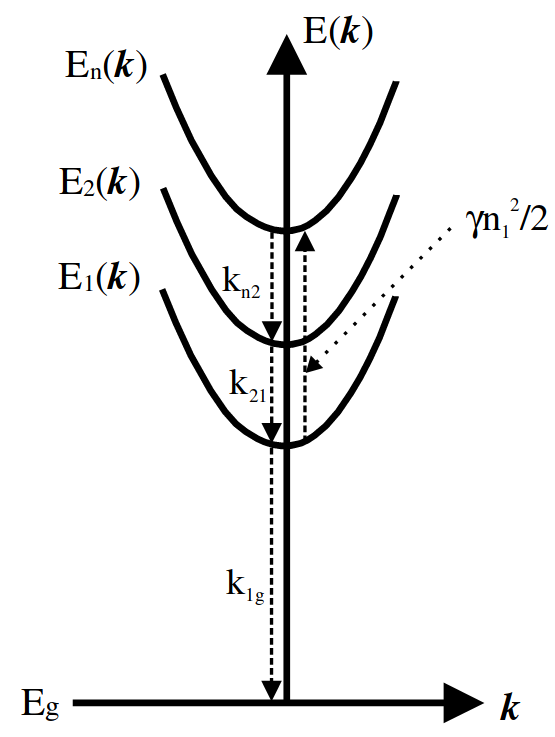
\includegraphics[scale=0.3]{images/chapter_prior_works/exciton_schematic_ma_2005}
	\caption{Schematic model of exciton-exciton annihilation in SWCNTs by Ma \textit{et al}.\ \cite{ma2005femtosecond}. Here, $E_\text{i}(\mathbf{k})$ and $E_\text{g}$ represent the $i$-th exciton band and the ground state, respectively. In addition, $\mathbf{k}$ denotes the exciton center-of-mass momentum. The parameter $k_\text{ij}$ indicates the linear relaxation rate from the $i$-th band to the $j$-th band. Finally, the rate of exciton-exciton annihilation is given as $\gamma n_1^2/2$, where a population of  $n_1$ excitons located within the $E_1(\mathbf{k})$ conduct exciton-exciton annihilation to produce a new exciton in a higher energy state. Reproduced from Ref.\ \cite{ma2005femtosecond}.}
	\label{fig:exciton_schematic_ma}
\end{figure}


Equation \eqref{eq:ma_n2} indicates that $n_2(t) \propto n_1^2(t)$. Indeed, the experimental data shown in Figure \ref{fig:abs_ma_2005}(a) appears to corroborate this. This plot shows the transient absorption response of (8,5) nanotubes probed at $E_{11}$ (953 nm) and $E_{22}$ (660 nm) states after the sample was resonantly excited at the $E_{11}$ photon energy. The square of the normalized transient absorption response measured at $E_{11}$ matches the dynamics of the normalized response recorded at $E_{22}$.

\begin{figure}[H]
 \centering
 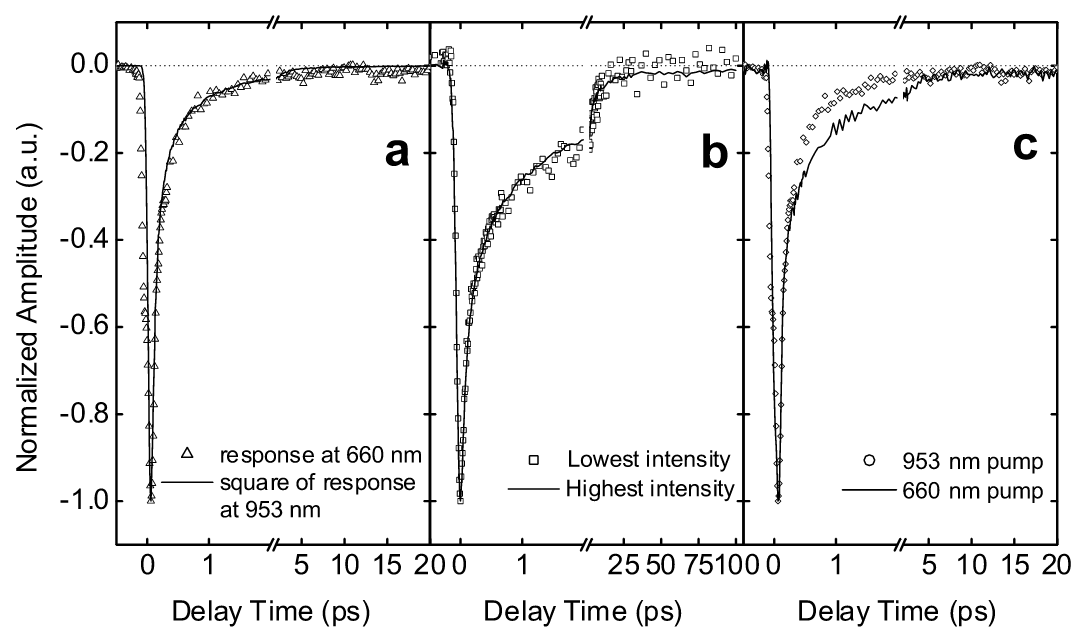
\includegraphics[scale=0.35]{images/chapter_prior_works/abs_ma_2005}
 \caption{(a) Differential absorption probed at 660 nm ($E_{22}$, triangles) and the square of the response ($[ \Delta A / A ]^2$) measured at 953 nm ($E_{11}$, solid line) after the sample was resonantly photoexcitined at $E_{11}$. (b) Differential absorption  measured at $E_{11}$ after the sample was resonantly excited at $E_{11}$ at a low (squares) and a relatively high (solid line) pump fluence. The fluences in the ``low'' and ``high'' scenarios differ by a factor of 17. (c) Differential absorption probed at $E_{22}$ after the sample was resonantly photoexcited at $E_{11}$ (cirles) and $E_{22}$ (solid line). The dynamics shown in (a) $-$ (c) are normalized at the signal maxima. All optical resonances here correspond to those of (8,5) nanotubes. Reproduced from Ref.\ \cite{ma2005femtosecond}.}
 \label{fig:abs_ma_2005}
\end{figure}

Strangely, they did not observe nonlinear carrier relaxation dynamics occuring at $E_{11}$ after resonantly exciting at $E_{11}$. Figure \ref{fig:abs_ma_2005}(b) demonstrates this. Both transient absorption curves taken at the highest and lowest fluences, which differ by a factor of 17, show similar decay rates. Also, they do acknowledge that Equation \eqref{eq:exciton_anih_ma_2005} provides good fits to the data, but only at very early times where $k_\text{1g} t \ll 1$ and for relatively high excitation fluences. Under these conditions, Equation \eqref{eq:exciton_anih_ma_2005} becomes
\begin{equation}
		n_1(t) = \frac{e^{-k_\text{1g}t}}{\gamma\cdot(1 - e^{-k_\text{1g}t} )/2k_\text{1g}}.
\end{equation}
However, a second exponential decay must be added to describe dynamics occuring at longer time delays. They attribute this to carrier dynamics detected from other nanotube species in the sample.

 Figure \ref{fig:abs_ma_2005}(c) shows the dynamics probed at the $E_{22}$ transition after the sample was photoexcited at both $E_{11}$ and $E_{22}$. When the sample was resonantly excited at $E_{11}$, absorption bleaching occurred at $E_{22}$ presumably because of exciton-exciton annihilation that causes a finite population of excitons at the $E_{22}$ energy level. A similar effect occurred when the sample was resonantly excited at $E_{22}$ after accounting for the fast $E_{22}$ to $E_{11}$ relaxation process demonstrated by Manzoni \textit{et al}. \cite{manzoni2005intersubband}. However, a notable difference in the carrier dynamics appeared at time delays greater than 300 fs. In particular, carrier relaxation occurred more slowly when the sample was excited at $E_{22}$ than at $E_{11}$. Ma \textit{et al}.\ claimed that this may be either due to the effect of exciting other nanotube species that are not specifically (8,5) nanotubes. They also suggested that $E_{22}$ excitons may also be initially relaxing into other intermediate energy levels such as the free-electron continuum states that are expected to exist between the $E_{11}$ and $E_{22}$ transitions.



\subsection{Diffusion-Limited Exciton-Exciton Annihilation}
The previous studies presenting evidence of exciton-exciton annihilation relied on models that implicitly assumed that excitons diffuse within a 3-D system \cite{wang2004observation,ma2004ultrafast, ma2005femtosecond}. This naturally conflicts with the understanding that carbon nanotubes effectively confine electrons to move in only one dimension. In fact, the rate of diffusion processes certainly depends on the dimensionality, $d$, of the system. The decay constant associated with exciton-exciton annihilation is time-independent only in cases where $d \geq 2$ \cite{valkunas2006exciton}. For 1-D systems, the annihilation rate assumes the form $\gamma = \gamma_0 / t^{-1/2}$ that yields the rate equation
\begin{equation}
		\frac{\mathrm{d} n_\text{ex}^2(t)}{\mathrm{d}t} = -\frac{1}{2 \sqrt{t}}  \gamma_0 \cdot n_\text{ex}^2(t),
		\label{eq:exc_1d_annih}
\end{equation}
whereas the rate equation given by Equation \eqref{eq:rate_eq_exc_anih} assumes that diffusion occurs in a 3-D system \cite{suna1970kinematics}. This difference emerges from the fact that a particle executing a 3-D random walk will return to its origin position with a probabilty of 0.35, whereas in dimensions less than or equal to 2 this probability is approximately unity \cite{suna1970kinematics}. As a result, the decay constant reduces with time for the 1-D case.

This discussion also requires the consideration of a key detail: the ratio between the Bohr radius of excitons and the size of the system, that is, the length scales of SWCNTs. In fact, exciton-exciton annihilation can exist in two regimes \cite{valkunas2006exciton}. On one hand, if exciton sizes are comparable to that of the system then the exciton-exciton annihilation rate should only depend on the rate at which two neighboring excitons interact with each other \cite{valkunas2006exciton}. For this case, Equation \eqref{eq:exc_1d_annih} would not be applicable as it assumes that exciton-exciton annihilation is limited by exciton diffusion. Instead, exciton-exciton annihilation occurs immediately after excitons are created \cite{valkunas2006exciton}. This can be described as coherent exciton-exciton annihilation \cite{valkunas2006exciton}.

On the other hand, if excitons are much smaller than the system they inhabit, then excitons must migrate until they reach another exciton before exciton-exciton annihilation occurs \cite{valkunas2006exciton}. In this scenario, the rate of exciton-exciton annihilation depends on both the diffusion rate of excitons as well as the annihilation rate of excitons in close proximity with each other \cite{valkunas2006exciton}. Hence, this regime is often referred to as diffusion-limited exciton-exciton annihilation.

The solution to the revised rate equation presented in Equation \eqref{eq:exc_1d_annih} is given as
\begin{equation}
	\frac{n_\text{ex}(0)}{n_\text{ex}(t)} = 1 + n_\text{ex}(0) \gamma_0 \sqrt{t},
\end{equation}
where $n_\text{ex}(t)$ denotes the time-dependent density of excitons and $\gamma_0$ represents a decay constant associated with exciton-exciton annihilation \cite{valkunas2006exciton}. Valkunas \textit{et al}.\ (2006) \cite{valkunas2006exciton} remarked that this solution does not correspond very well to the experimental data measured by Wang \textit{et al}.\ \cite{wang2004observation} and Ma \textit{et al}.\ \cite{ma2004ultrafast, ma2005femtosecond}. In those studies, the models fit to the data very well by assuming that the exciton-exciton annihilation rate does not depend on time. For this reason, Valkunas \textit{et al}.\ \cite{valkunas2006exciton} argued that diffusion-limited exciton-exciton annihilation is not the correct interpretation of those results. They claimed that it must be the case that exciton sizes are on the order of typical nanotube lengths so that the effects of diffusion ought to be negligible.

Instead, they studied carrier dynamics using a stochastic model depicted in Figure \ref{fig:exciton_manif_valkunas}. Their model is motivated by the understanding that excitons occupying a set of multiexciton states, denoted as [ $i$ ], can access another group of excited states, represented as [ $\displaystyle\bar{i}$ ], after undergoing exciton-exciton annihilation. Here, the parameter $\Gamma_{i \rightarrow \bar{i}-1}$ determines the rate of exciton-exciton annihilation which causes a transition from the $i$-th manifold to manifold labeled as $\bar{i} - 1$. The term $K_{i \rightarrow \bar{i}}$ characterizes carrier relaxation rates due to phonon scattering. Finally, $k_i$ indicates a linear relaxation rate within the $i$-th manifold and the terms $G(t)$ and $\bar{G}(t)$ are rates of exciton generation due to the optical pump.

\begin{figure}[H]
	\centering
	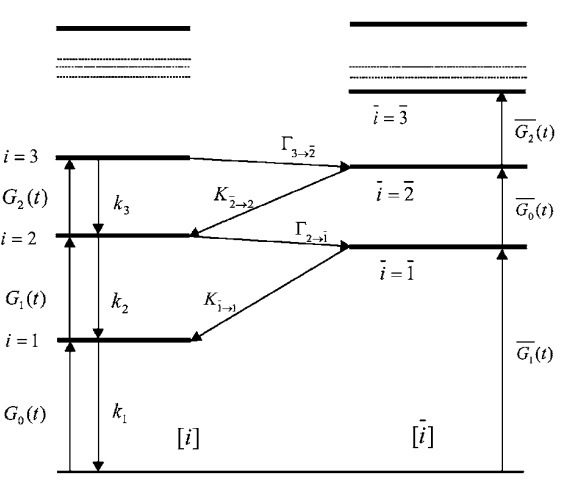
\includegraphics[scale=0.5]{images/chapter_prior_works/exciton_manifold_valkunas_2006}
	\caption{Exciton-exciton annihilation model proposed by Valkunas \textit{et al}.\ (2006) \cite{valkunas2006exciton}. Here, the states in which excitons undergo exciton-exciton annihilation include a manifold of multiexciton states (left, grouped as [ $i$ ]) and another manifold associated with higher energy excited states that can be accessed via exciton-exciton annihilation (right, grouped as [ $\bar{i}$ ]). The terms $G_{i}(t)$ and $\bar{G_{i}}(t)$ determine the rates of exciton generation from the $i$-th and $\bar{i}$-th manifolds respectively. Furthermore, $\Gamma_{i \rightarrow \bar{i}-1}$ and $K_{i \rightarrow \bar{i}}$ refer to relaxation rates occuring between these manifolds. Finally, the parameter $k_\text{i}$ indicates the linear relaxation rate from the $i$-th to the $i-1$-th energy level. Reproduced from Ref.\ \cite{valkunas2006exciton}. }
	\label{fig:exciton_manif_valkunas}
\end{figure}

Despite the extent at which exciton states are abstracted in this scheme, Valkunas \textit{et al}.\ remarked that only the $E_{11}$ and $E_{22}$ energy levels need to be considered to adequately explain experimental data. The exciton populations within the $E_{11}$ and $E_{22}$ can be matched with the total populations of the [ $i$ ] and [ $\bar{i}$ ] manifolds respectively \cite{valkunas2006exciton}. The key difference in their model from that of Ma \textit{et al}.\ (2005) \cite{ma2005femtosecond} is that they account for the fast intersubband relaxation demonstrated by Manzoni \textit{et al}.\ (2005) \cite{manzoni2005intersubband} by using the parameter $K_{i \rightarrow \bar{i}}$.
From this approach, they demonstrated that their model qualitatively agrees with the results presented by Ma \textit{et. al}.\ (2005), \cite{ma2005femtosecond} as shown in Figure \ref{fig:e11_e22_pop_valkunas}. Here, the model predicts that the population of $E_{22}$ excitons varies with the square of the population of $E_{11}$ excitons, which agrees with the observations of Ma \textit{et al}.\ (2005) \cite{ma2005femtosecond}.

\begin{figure}[H]
	\centering
	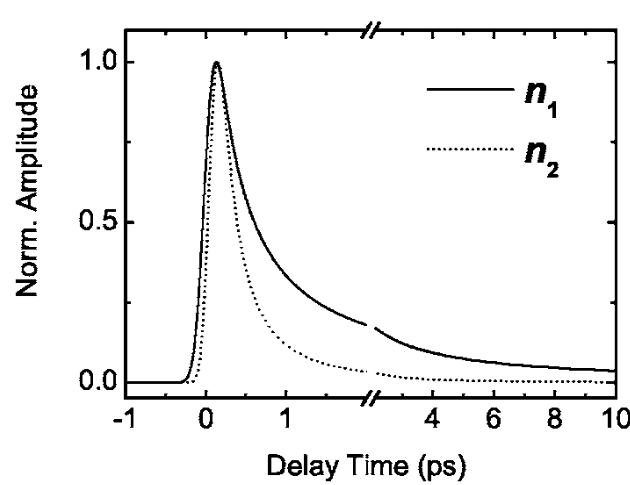
\includegraphics[scale=0.4]{images/chapter_prior_works/e11_e22_population_valkunas_2006}
	\caption{Time evolution of exciton populations within the $E_{11}$ and $E_{22}$ energy level denoted as $n_1$ and $n_2$ respectively as predicted by the stochastic model presented by Valkunas \textit{et al} \cite{valkunas2006exciton}. The authors state that this model reproduces the $n_2(t) \propto (n_1(t))^2$ behavior observed by Ma \textit{et al}.\ (2005) \cite{ma2005femtosecond}. Reproduced from Ref.\ \cite{valkunas2006exciton}. }
	\label{fig:e11_e22_pop_valkunas}
\end{figure}

In contrast with these previous findings, Luer \textit{et al}.\ (2009) provided experimental evidence showing that exciton-exciton annihilation in SWCNTs is indeed diffusion-limited and can be modeled using the appropriate 1-D decay constant presented in Equation \eqref{eq:exc_1d_annih} \cite{luer2009size}. They studied carrier dynamics in (6,5)-enriched SWCNTs that were individually suspended in a film using a xerogel \cite{luer2009size}. Figure \ref{fig:dtt_luer_2009} presents transient absorption data and a schematic of their model that can be expressed as a set of rate equations
%
\begin{equation}
	\begin{split}
			\frac{\mathrm{d} N_1}{\mathrm{d} t} &= -k_{10} t^{\alpha} N_1 - k_\text{a}N_1^2 + k_{21} N_1,
			\\
			\frac{\mathrm{d} N_2}{\mathrm{d} t} &= \frac{1}{2} k_\text{a} N_1^2 - k_{21} N_1
	\end{split}
\end{equation}
%
where $N_1$ and $N_2$ denote exciton densities within the first ($E_{\text{x}_1}$) and second ($E_{\text{x}_2}$) subbands, respectively. The exciton-exciton annihilation rate is given as $k_\text{a} = k_\text{a}^* t^{-1/2}$. Here, it is assumed that annihilation occurs immediately when two excitons make sufficient contact with each other. The variable $k_\text{a}^*$ also gives the exciton diffusion rate $D_\text{exc}$ via the expression
\begin{equation}
	k_\text{a}^* = \sqrt{32 D_\text{exc}/ \pi},
	\label{eq:exc_anih_diffuse_luer_2009}
\end{equation}
a result which was verified using Monte Carlo simulation of diffusion-limited exciton-exciton annihilation on a 1-D chain. Based on the findings of Manzoni \textit{et al}.\ (2005) \cite{manzoni2005intersubband}, $k_{21} = 2.3 \times 10^{13}$ \si{\per\second} represents the relaxation rate from $ E_{\text{x}_2} $ to $E_{\text{x}_1}$. Finally, $k_{1} = k_{10}t^\alpha $ indicates the relaxation rate from $E_{\text{x}_1}$ to ground state with exponent $\alpha$.

Fits of the model to the experimental data gave a time-dependent annihilation constant of $k_\text{a}(t) = 1.0 \times 10^7 \text{nm } \text{s}^{-1/2} \cdot t^{-1/2}$. However, Figure \ref{fig:dtt_2_luer_2009} demonstrates that Luer \textit{et al}.\ \cite{luer2009size} did not observe strong evidence for efficient exciton-exciton annihilation. The normalized transient absorption curves do not appear to show a dominant early decay process that becomes drastically faster as the pump fluence increases.

\begin{figure}[H]
	\centering
	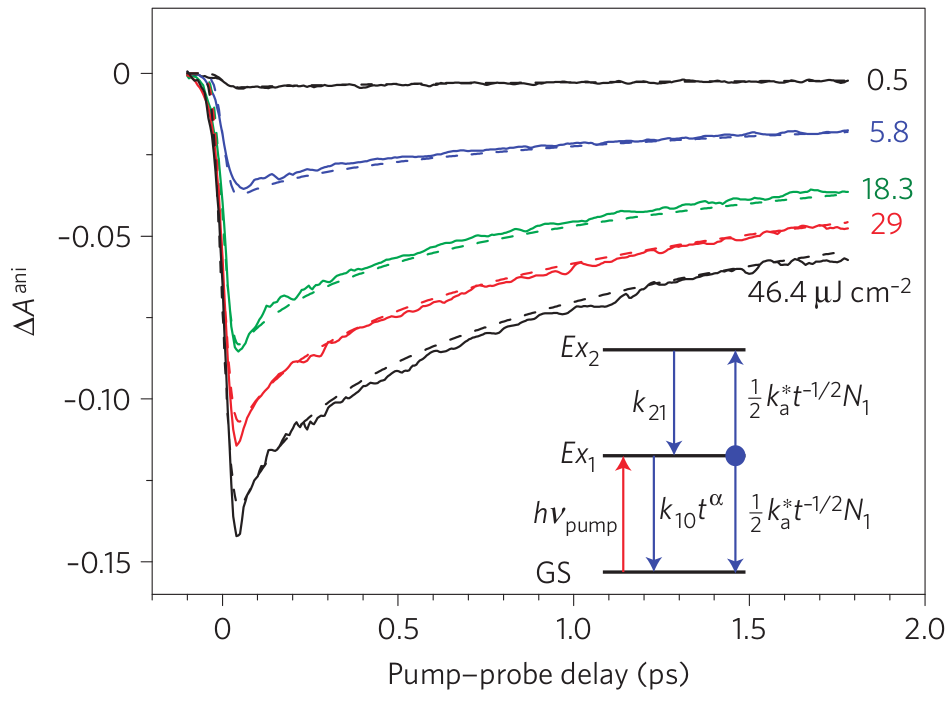
\includegraphics[scale=1.2]{images/chapter_prior_works/dtt_2_luer_2009}
	\caption{Differential absorption probed at the $E_{11}$ transition of (6,5) nanotubes presented with labeled pump fluences (\si{\micro \joule} \si{\cm^{-2}}). The pump and probe pulses were centered at photon energies of 1.29 eV and 1.24 eV, respectively, and were polarized parallel to each other. Here, the (6,5) $E_{11}$ resonance is at 1.24 eV. The dashed lines correspond to fits produced from the kinetic model shown in the inset. Excitons in first subband $E_{\text{x}_1}$ created by an optical pump of photon energy $h \nu_\text{pump}$ and undergo exciton-exciton annihilation at a time-dependent rate $k_\text{a}^* t^{-1/2}$, which creates a population of excitons in the second subband $E_{\text{x}_2}$. The variables $k_{21}$ and $k_{10}t^{\alpha}$ represent, respectively, decay rates from $E_{\text{x}_2}$ to $E_{\text{x}_1}$ and $E_{\text{x}_1}$ to the ground state. Reproduced from Ref.\ \cite{luer2009size}.}
	\label{fig:dtt_luer_2009}
\end{figure}

\begin{figure}[ht]
	\centering
	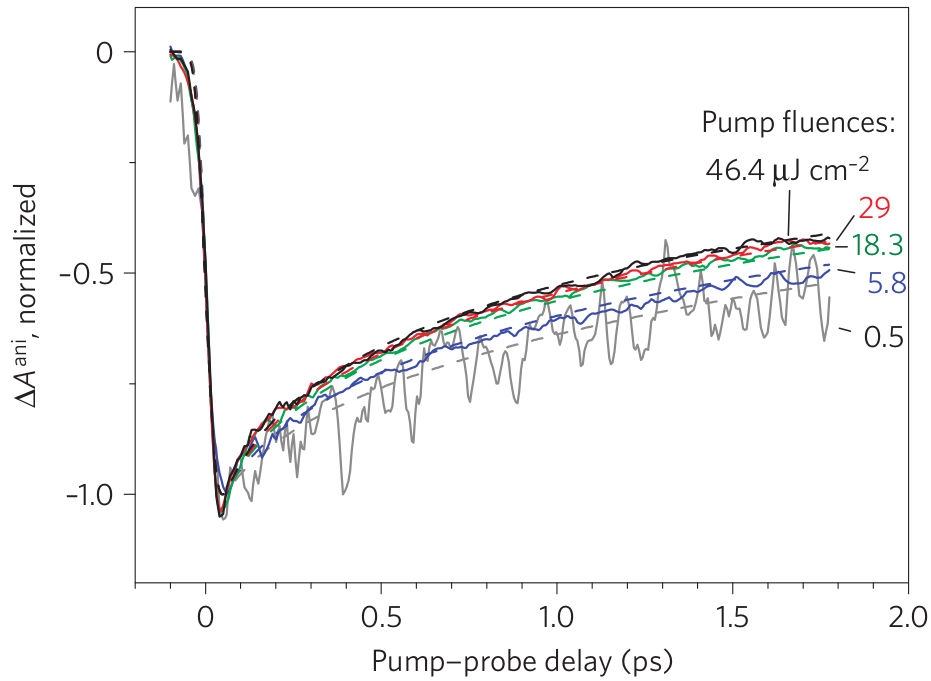
\includegraphics[scale=1.2]{images/chapter_prior_works/dtt_3_luer_2009}
	\caption{Normalized transient aborption data taken from Figure \ref{fig:dtt_luer_2009}. The relaxation dynamics do not appear to show a strong depdence on pump fluence. Hence, exciton-exciton annihilation is said to be an inefficient process in this scenario. Reproduced from Ref.\ \cite{luer2009size}.}
	\label{fig:dtt_2_luer_2009}
\end{figure}

Luer \textit{et al}.\ \cite{luer2009size} also estimated the size of excitons occuring in (6,5) SWCNTs using the well-known phase-space filling model \cite{schmitt1985theory, greene1990all}. According to this model, the relative change in oscillator strengths of excitonic resonances occurs as a result of the Pauli exclusion principle. Indeed, this change in the oscillator strength $\delta f_\text{}/ f_\text{}$ depends on the momentum-space distribution functions $f_\text{e}(k)$ and $f_\text{h}(k)$ of electrons and holes respectively, and is therefore written as
\begin{equation}
	\frac{\delta f_\text{}}{f_\text{}} = - \sum_{k} \left\{ \frac{ [ f_\text{e}(k) + f_\text{h}(k)] \tilde{\Psi}_\text{exc}(k)}{\Psi_\text{exc}(x=0)} \right\},
	\label{eq:osc_strength}
\end{equation}
which also includes the exciton wavefunction $\Psi_\text{exc}$ as well as its corresponding Fourier transform $\tilde{\Psi}_\text{exc}$.

For electrons and holes that pair together to form excitons, the distribution functions are given as
%
\begin{equation}
	f_\text{e}(k) = f_\text{h}(k) = \frac{N}{2} | \tilde{\Psi}_\text{exc}(k)|^2,
\end{equation}
%
where $N$ refers to the density of excitons per unit length. In this expression, excitons represent a linear combination of single-particle, fermionic states distributed according to $\tilde{\Psi}_\text{exc}(k)$ \cite{schmitt1985theory}. Therefore, the formation of an exciton must correspond to an occupation probability in the fermion phase space $|\tilde{\Psi}_\text{exc}(k)|^2$ \cite{schmitt1985theory}. This probability is equally shared between spin-up and spin-down states, which explains the factor of 1/2 \cite{schmitt1985theory}.

The exciton wavefunction $\Psi_\text{exc}$ can be approximated as
\begin{equation}
	\Psi_\text{exc}(x) = \left( \sqrt{a \sqrt{\pi}} \right)^{-1} \exp[-x^2 / (2 \xi^2_\text{e})],
\end{equation}
where $\xi_\text{e}$ represents the electron-hole correlation length, otherwise known as the exciton size \cite{capaz2006diameter}. Using this wavefunction, Equation \eqref{eq:osc_strength} becomes
%
\begin{equation}
	\frac{\delta f}{f} = - N \gamma \xi_\text{e}, \hspace{4mm} \gamma \approx 2.05.
\end{equation}
%
Here, $\gamma$ is a proportionality constant that varies with the wavefunction used to perform this calculation. Certainly, the relative change in the oscillator strength is related to the differential absorption $\Delta A / A$ as well as a saturation density $N_\text{s}$ by the expression
\begin{equation}
	\frac{\delta f}{f} = \frac{\Delta A}{A} = \frac{N}{N_\text{s}},
\end{equation}
where $N_\text{s}^{-1} = \gamma \xi_\text{e}$. Starting from this expression, Luer \textit{et al}.\ argued that the change in absorption $\Delta A$ can be derived as
\begin{equation}
	\Delta A = -r_\text{a} \gamma \sigma_\text{C} \frac{\xi_\text{e}}{\xi_\text{C}} I_\text{abs}.
	\label{eq:abs_exc_len}
\end{equation}
This includes new paramaters defined as $\sigma_\text{C} = 7 \times 10^{-18}$ \si{\cm\squared}, the absorption cross-section of nanotubes determined in an earlier study \cite{zheng2004solution}, $\xi_\text{C} = 0.01$ nm, which denotes the atom density of a (6,5) nanotube, $I_\text{abs}$, which characterizes absorbed photons per unit area, and $r_{a}$, which represents a correction factor used to account for the fact that some individually suspended nanotubes will not be aligned parallel to the polarization of the incident optical pump beam.

\begin{figure}[ht]
	\centering
	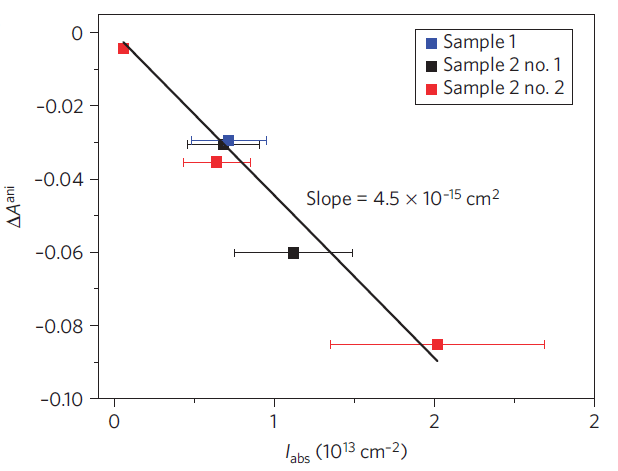
\includegraphics[scale=0.8]{images/chapter_prior_works/exciton_size_fit_luer_2009}
	\caption{Maximum differential absorption as a function of the absorbed pump fluence $I_\text{abs}$. The solid line represents a linear regression using the function defined in Equation \eqref{eq:abs_exc_len}, which was used to obtain an exciton size of $\xi_\text{e} = 2.0 \pm 0.7$ nm. Reproduced from Ref.\ \cite{luer2009size}.}
	\label{fig:lin_fit_luer_2009}
\end{figure}

Luer \textit{et al}.\ used Equation \eqref{eq:abs_exc_len} to obtain an estimate of the exciton size. For this, they measured the maximum change in absorption as a function of pump fluence as shown in Figure \ref{fig:lin_fit_luer_2009}. After perfoming a linear fit on this data, they obtained an exciton size of $2.0 \pm 0.7$ nm, which agrees with theoretical expectations \cite{spataru2004excitonic, chang2004excitons, tretiak2007excitons} as well as the estimate by Ostojic \textit{et al}.\ (2005) \cite{ostojic2005stability}. From Equation \eqref{eq:exc_anih_diffuse_luer_2009}, they obtained a diffusion length less than 10 nm, which happens to be an order of magnitude less than the corresponding value obtained in fluorescence measurements \cite{cognet2007stepwise}. These results, combined with the inefficient exciton-exciton annihilation that they observed, led Luer \textit{et al}.\ \cite{luer2009size} to conclude that transient absorption spectroscopy probes the total population of excitons, many of which are short-lived and do not directly participate in exciton-exciton annihilation due to their shorter diffusion lengths. They suggested that time-resolved fluoresence measurements appear to probe long-lived excitons that have higher diffusion lengths and are therefore more likely to engage in exciton-exciton annihilation processes.

\begin{figure}[ht]
	\centering
	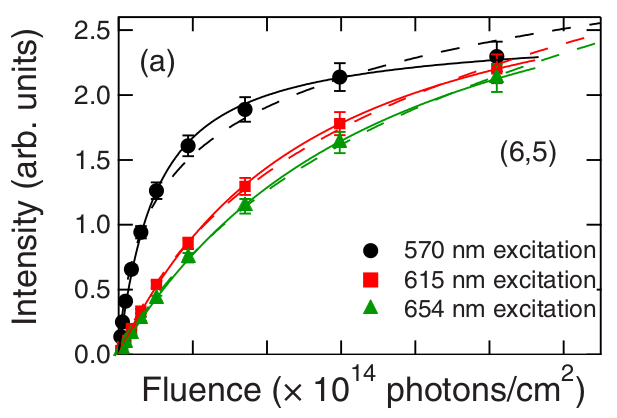
\includegraphics[scale=1.9]{images/chapter_prior_works/murakami_pl_saturation}
	\caption{Time-integrated photoluminescence intensity of (6,5) nanotubes shown as a function of optical pump fluence. The solid and dashed lines correspond to fits using, respectively, the diffusion-limited exciton-exciton annihilation proposed by Murakami and Kono as well as a model based on the conventional rate-equation in Equation \eqref{eq:rate_eq_exc_anih}. Regardless of the excitation wavelength, photoluminescence appears to saturate at higher pump fluences. Murakami and Kono interpreted this as evidence of exciton-exciton annihilation, establishing an upper limit on the population of photoexcited excitons. Reproduced and modified from Ref.\  \cite{murakami2009existence}. }
	\label{fig:pl_saturation_murakami}
\end{figure}

 Indeed, this hypothesis is plausible as a majority of the strong evidence in support of highly efficient exciton-exciton annihilation processes in SWCNTs has been primarily derived from photoluminescence measurements. As another example of this, Murakami and Kono (2009) showed that light emission from nanotubes appears to saturate at higher optical pump fluences, as shown in Figure \ref{fig:pl_saturation_murakami} \cite{murakami2009existence}. They also attributed this phenomenon to the effect of diffusion-limited exciton-exciton annihilation, claiming that this process sets an upper limit on the number of excitons that can be created. In spite of this, transient absorption measurements appear to suggest that if indeed exciton-exciton annihilation occurs, it is not necessarily the most dominant carrier relaxation process \cite{ostojic2004interband, manzoni2005intersubband, luer2009size}. Other nonradiative processes will have to be accounted for to obtain a comprehensive understanding of the ultrafast carrier dynamics of SWCNTs.

%\section{Possible Presence of Bi-excitons and Trions}

%non-degenerate pump-probe. Amplified Ti:sapphire laser operating at 200 KHz and pulse duration of 100 fs. Probe generated using supercontinuum generation in a sapphire crystal. Pump generated using optical parametric amplifier (OPA). Studied a (6,5)-enriched dispersion. Figure \ref{fig:abs_yuma} shows linear absorption spectrum of sample.

%\begin{figure}[ht]
%	\centering
%	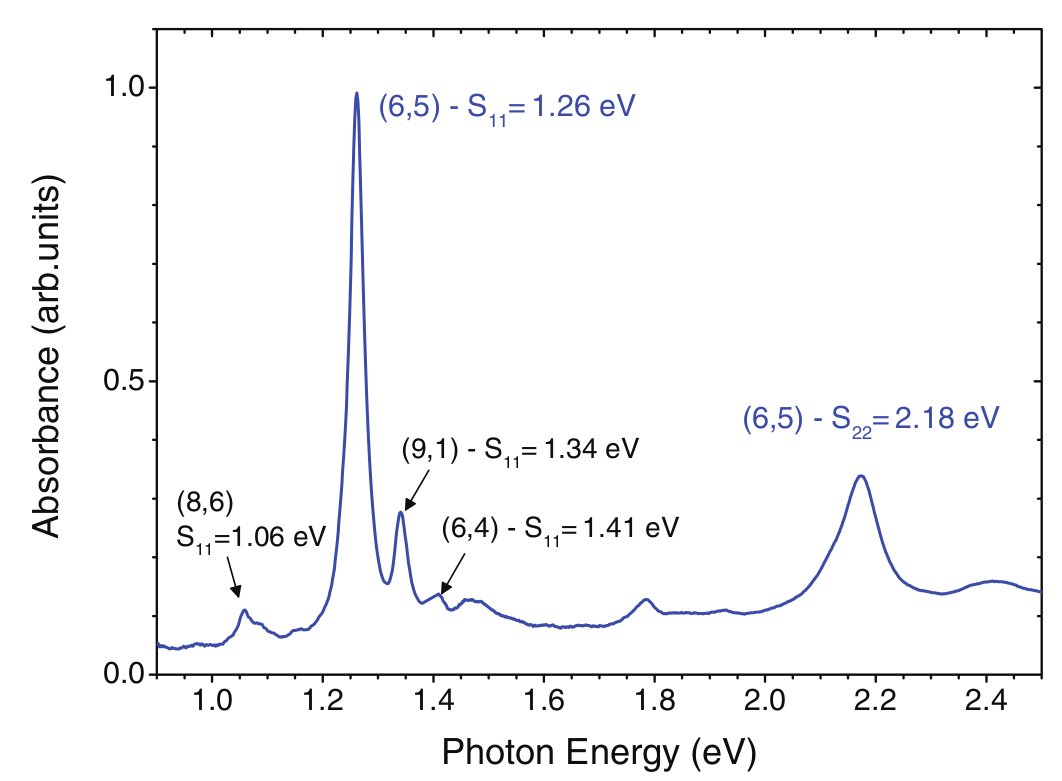
\includegraphics[scale=0.3]{images/chapter_prior_works/abs_yuma}
%	\caption{Slightly different nomenclature. Here, $S_\text{ij} \equiv E_\text{ij}$.  Reproduced from Ref.\ \cite{yuma2013biexciton}.}
%	\label{fig:abs_yuma}
%\end{figure}

%Figure \ref{fig:dtt_yuma} shows experimental data after resonantly exciting $E_{22}$ transition of (6,5) nanotube. Notice photobleaching and a blue shift occuring at $E_{11}$ peak. Interpreted as excitons occupying $E_{11}$ states. Charge screening due to Coulomb interactions between excitons blueshifts exciton peak. State that initial sharp decay due to exciton-exciton annihilation.

%Observed photo-induced absorption at 1.13 eV. Attribute this to the formation of biexcitons. Provided additional evidence by pumping at and below $E_{11}$. When pumping below $E_{11}$, photo-induced absorption at 1.13 eV recedes. When pumping $E_{11}$ resonantly, photo-induced absorption becomes more significant indicating that it may be directly associated with (6,5). Carrier dynamics at $E_{11}$ and bi-exciton appear to be correlated with each other.

%\begin{figure}[ht]
%	\centering
%	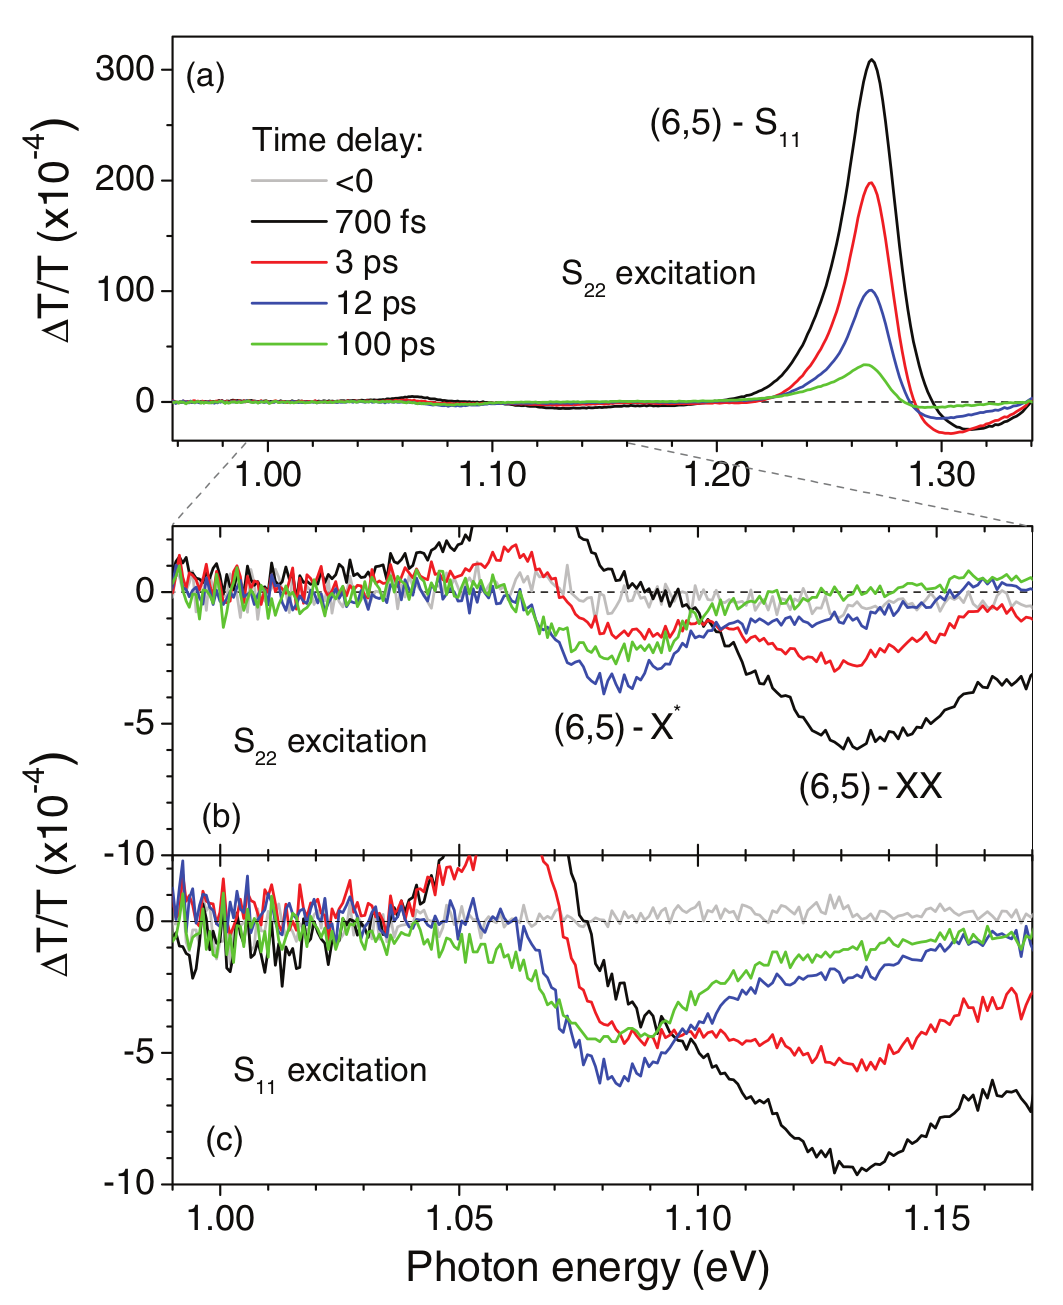
\includegraphics[scale=0.3]{images/chapter_prior_works/dtt_yuma}
%	\caption{{\color{red} UNFINISHED} Reproduced from Ref.\ \cite{yuma2013biexciton}.}
%	\label{fig:dtt_yuma}
%\end{figure}


%Exciton-Exciton annihilation \cite{valkunas2006exciton, yuma2013biexciton}.
%They also show that exciton-exciton annihilation occurs over a time scale such that it is hard to reach Mott densitty of excitons where excitons immediately dissociate to form plasma of free carriers. These a
%Apparently, excitons dissociate into free electron-hole pairs before recombination occurs \cite{kumamoto2014spontaneous}.

One confounding variable in this discussion is how the dielectric environment of the SWCNTs affects carrier relaxation. As discussed in Section \ref{section:dielectric_screening}, the dielectric envrionment in which SWNCTs are immersed can affect optical resonances. An environment with a higher dielectric constant $\varepsilon_\text{env}$ will screen electron-electron interactions, which will cause the resonances to redshift further as this dielectric constant increases. This should also have some effect on the Mott density of SWCNTs. As the dielectric constant of the environment increases, the Mott density should correspondingly decrease as a smaller population of excitons would be needed to completely negate the Coulomb interaction between electrons and holes. To the best of our knowledge, this has not yet been fully explored in SWCNTs within the current literature. However, one relevant study was conducted by Ohno \textit{et al}.\ (2007) \cite{ohno2007excitonic}.

Ohno \textit{et al}.\ \cite{ohno2007excitonic} performed time-resolved photoluminescence measurements on (9,7) SWCNTs that were directly grown over trenches. The setup that they used was designed to measure a time-domain correlation signal. Here, the output of a Ti:sapphire laser (100 fs, 80 MHz, 1.55 eV) was split into two arms. The two arms were modulated by an optical chopper at frequencies $f_1$ and $f_2$, respectively. Furthermore, a delay stage was used to alter the optical path length of one arm. Both beams were focused onto the sample and the photoluminescence signal measured at frequency $f_1 - f_2$ was obtained using a lock-in amplifier together with a monochromator.

They studied the dynamics of photoluminescence under two conditions \cite{ohno2007excitonic}. In one instance, the SWCNTs were immersed in ambient air ($\varepsilon_\text{env} = 1$). For another experiment, the SWCNTs were instead immersed in hexane ($\varepsilon_\text{env} = 1.9$), a solvent. Photoluminescence decayed much more slowly for the sample immersed in air than for the sample immersed in hexane, as shown in Figure \ref{fig:dtt_ohno}. For the sample immersed in air, the dynamics corresponded to a bi-exponential fit. In this case, the fast and slow decay constants were reported as 26 and 293 ps, respectively. However, for the sample immersed in hexane, only a \textit{single} exponential, corresponding to a decay of 5.1 ps, could be fit to the data.


In explaining this, Ohno \textit{et al}.\ speculated that nonradiative recombination centers may be created on the surfaces between the SWCNTs and the solvent \cite{ohno2007excitonic}. However, the very fast decay for the sample in hexane may also be a sign of highly efficient exciton-exciton annihilation, although it is not quite clear why the dielectric environment would enhance exciton-exciton annihilation processes. Unfortunately, Ohno \textit{et al}.\ did not provide any data showing how these dynamics change with increasing pump intensity so this idea cannot be corrobrated by their study \cite{ohno2007excitonic}.

\begin{figure}[H]
	\centering
	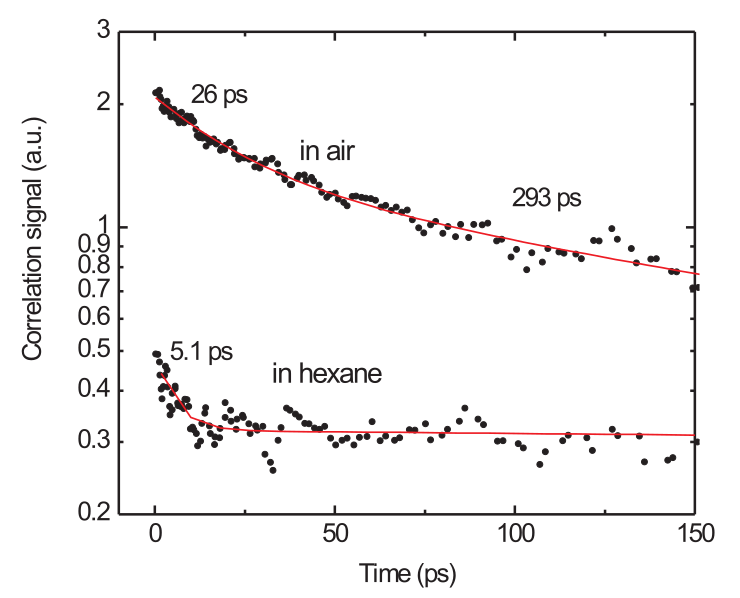
\includegraphics[scale=0.4]{images/chapter_prior_works/dtt_ohno}
	\caption{Time-domain correlation signal of (9,7) SWCNTs immersed in air and in hexane, as reported by Ohno \textit{et al}.\ \cite{ohno2007excitonic}. The solid curves correspond to fits to the data using bi-exponential functions. For the sample immersed in air, the fast and slow decay components were given as 26 and 293 ps, respectively. For the sample immersed in hexane, only a fast component of 5.1 ps was obtained. Reproduced from Ref.\ \cite{ohno2007excitonic}. }
	\label{fig:dtt_ohno}
\end{figure}


\section{The Optical Stark Effect}
\label{sec:optical_stark_effect}

The optical Stark effect describes a coherent process that only occurs during the presence of an intense optical pump beam. In such processes, the phase of the induced polarization becomes correlated to that of the incident light \cite{shah1996ultrafast}. Figure \ref{fig:optical_stark_effect_schematic_sie} shows a schematic diagram of this phenomenon. Here, the states $\ket{a}$ and $\ket{b}$ represent the ground state and an excited state of a two-level system and $E_0$ denotes the energy difference between these states. Light-matter coupling introduced by optical pump of photon energy $h \nu$ creates the virtual states $\ket{a + h \nu}$ and $\ket{b - h \nu}$ that repel the original equilibrium states. After this repulsion occurs, the energy splitting $\Delta E_\text{splitting}$ between $\ket{a}$  and $\ket{b - h \nu}$ as well as $\ket{b}$ and $\ket{a + h \nu}$ is given as
\begin{equation}
	\Delta E_\text{splitting} = \sqrt{\Delta^2 + (\hbar\Omega_\text{R})^2 },
\end{equation}
and parameterized by the detuning energy $\Delta = h \nu - E_0$ \cite{mysyrowicz1986dressed}. The variable $\Omega_\text{R}$ denotes the Rabi frequency and $\hbar \Omega = \mu E$, where $\mu$ and $E$ correspond to the transition dipole moment and the electric field of the pump, respectively
\cite{mysyrowicz1986dressed}. For sufficiently large negative detunings ($|\Delta| \gg \hbar \Omega_\text{R}$), the total change $\Delta E$ of the resonance energy $E_0$ can be expressed as

\begin{figure}[ht]
	\centering
	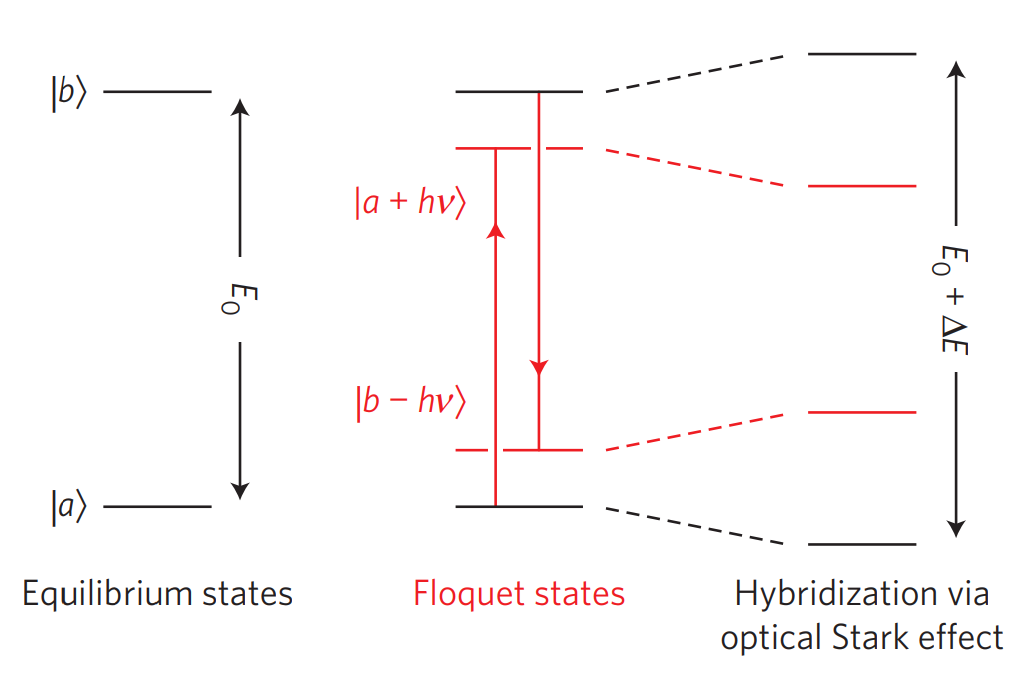
\includegraphics[scale=0.3]{images/chapter_prior_works/optical_stark_effect_sie_2014}
	\caption{Schematic diagram of the optical Stark effect. In equilbrium, the system contains two states $\ket{a}$ and $\ket{b}$ that have an energy difference of $E_0$. When an intense optical pump of energy $h \nu$ is introduced to the system, two new virtual states $\ket{a + h \nu }$ and $\ket{b - hv}$, also commonly known as Floquet states, emerge. These virtual states interact with the original equilibrium states, causing a shift in energy of the $E_0$ resonance energy. Reproduced from \cite{sie2015valley}.}
	\label{fig:optical_stark_effect_schematic_sie}
\end{figure}

%\begin{equation}
%		\Delta E = \sqrt{(\hbar \Omega_R)^2 + \Delta^2} - \Delta,
%\end{equation}

\begin{equation}
		\Delta E \propto \frac{\mu^2 I}{\Delta},
		\label{eq:ose_blueshift}
\end{equation}
where $I$ indicates the intensity of the optical pump \cite{combescot1992semiconductors}.

A large detuning energy is often needed to properly resolve the optical Stark effect in experiments. For example, in quantum well structures it has been observed that photoexcitations close to or above the band gap energy can create real carriers. The presence of real carriers photobleaches optical resonances and masks the presence of any coherent spectral shift induced by the optical Stark effect \cite{peyghambarian1984blue}. This poses a significant impediment for ultrafast optical switching applications using inorganic semiconductors as real carriers created in these systems relax to the ground state on a nanosecond timescale \cite{maeda2006gigantic}. SWCNTs surpass this limitation as they undergo carrier relaxation processes on a picosecond timescale \cite{ostojic2004interband, wang2004observation, manzoni2005intersubband, maeda2006gigantic}.

\begin{figure}[ht]
	\centering
	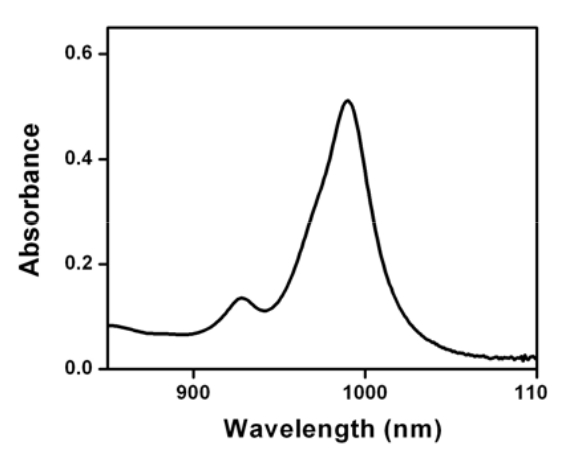
\includegraphics[scale=0.4]{images/chapter_prior_works/absorption_spectrum_song_2006}
	\caption{Absorption spectrum of the (6,5)-enriched SWCNTs that were individually suspended in heavy water ($\text{D}_2 \text{O}$) using single-stranded DNA \cite{zheng2003structure} and studied by Song \textit{et al}.\ (2006) \cite{song2006optical}. The spectrum shows the (6,5) $E_{11}$ resonance located at 990 nm (1.25 eV) as well as another peak which corresponds to a phonon sideband of (6,5) nanotubes. Reproduced from Ref.\  \cite{song2006optical}.}
	\label{fig:abs_song_2006}
\end{figure}

Song \textit{et al}.\ (2006) \cite{song2006optical} observed an optical Stark shift of the (6,5) $E_{11}$ resonance . Figure \ref{fig:abs_song_2006} shows an aborption spectrum of their (6,5)-enriched dispersion that they studied. This includes the (6,5) $E_{11}$ resonance at 990 nm (1.25 eV) as well as another peak corresponding a phonon sideband found in (6,5) nanotubes. With the optical pump detuned below the $E_{11}$ energy transition, the $E_{11}$ peak blueshifted, as shown in Figure \ref{fig:dtt_song_2006}. The red curve corresponds to the difference absorption spectrum $\Delta \alpha$ defined as
\begin{equation}
	\Delta\alpha(\omega) = \alpha^\text{P}(\omega) - \alpha^0(\omega),
\end{equation}
where $\alpha^\text{P}(\omega)$ and $\alpha^\text{0}(\omega)$ denote the absorption spectrum in the presence and absence of the strong optical pump, respectively. The blue curve expresses  the first derivative $\partial\alpha / \partial\omega$ of the absorption spectrum shown in Figure \ref{fig:abs_song_2006}.

\begin{figure}[ht]
	\centering
	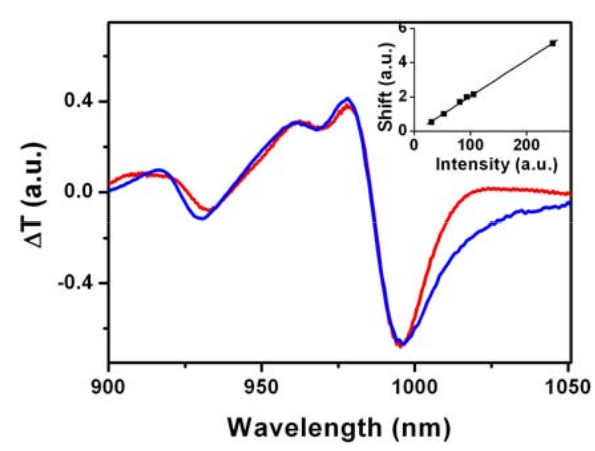
\includegraphics[scale=0.4]{images/chapter_prior_works/dtt_song_2006}
	\caption{Difference absorption spectrum $\Delta \alpha(\omega)$ measured after photoexciting at \SI{1.8}{\um} (0.69 eV) at a time delay when the pump and the probe arrive at the same time (red trace). For small spectral shifts, the differential absorption is expected to be proportional to the first derivative of the absorption spectrum (Figure \ref{fig:abs_song_2006}) with respect to the photon frequency. The inset figure shows that spectral shifts scale linearly with the intensity of the optical pump. Reproduced from \cite{song2006optical}.}
	\label{fig:dtt_song_2006}
\end{figure}

Given a spectral shift $\delta \omega$ induced by the optical Stark effect, Song \textit{et al}.\ noted that $\alpha^\text{P}(\omega) = \alpha^0 (\omega + \delta \omega)$. For relatively small frequency shifts, $\alpha^0 (\omega + \delta \omega)$ can be Taylor expanded to obtain the difference absorption spectrum
\begin{equation}
	\Delta \alpha(\omega) = \frac{\partial \alpha(\omega)}{\partial \omega} \cdot \delta\omega,
\end{equation}
which represents the first order term within the Taylor expansion. The good agreement between the red and blue curves in Figure \ref{fig:dtt_song_2006} confirms this. Furthermore, the inset figure within Figure \ref{fig:dtt_song_2006} also demonstrates that the spectral shift scales linearly with the optical pump intensity as expected by Equation \eqref{eq:ose_blueshift}.



Maeda \textit{et al}.\ (2006) also observed a coherent optical phenomenon, which they attributed to the optical Stark effect, within a film of SWCNT bundles containing both semiconducting and metallic nanotubes \cite{maeda2006gigantic}. Figure \ref{fig:abs_maeda_2006} shows an absorption spectrum $\alpha$ for this sample. It also reveals the change in absorption $\Delta \alpha$ at given time delay $t_\text{d}$ after the sample was photoexcited at 0.685 eV. At $t_\text{d} = 0.1$ ps, the absorption decreases significantly at 0.685 eV. However, the spectral width of the negative $\Delta\alpha$ is 40 meV, whereas the width of the absorption peak is about 200 meV.

This behavior marks a clear sign of a phenomenon known as spectral hole burning. Maeda \textit{et al}.\  noted that the resonance at 0.685 eV is inhomogenously broadened due to the presence of nanotubes with varying diameters \cite{maeda2006gigantic}. As a result, the optical pump resonantly excited only a subset of nanotubes whose optical responses become dominant in the $\Delta \alpha$ spectrum. The $\Delta \alpha$ spectrum at $t_\text{d} = 0.1$ ps also contains positive changes at 0.6 and 0.76 eV. In combination with the negative signal observed at 0.685 eV, this suggests that the optical resonance has temporarily split into two new states.

\begin{figure}[H]
	\centering
	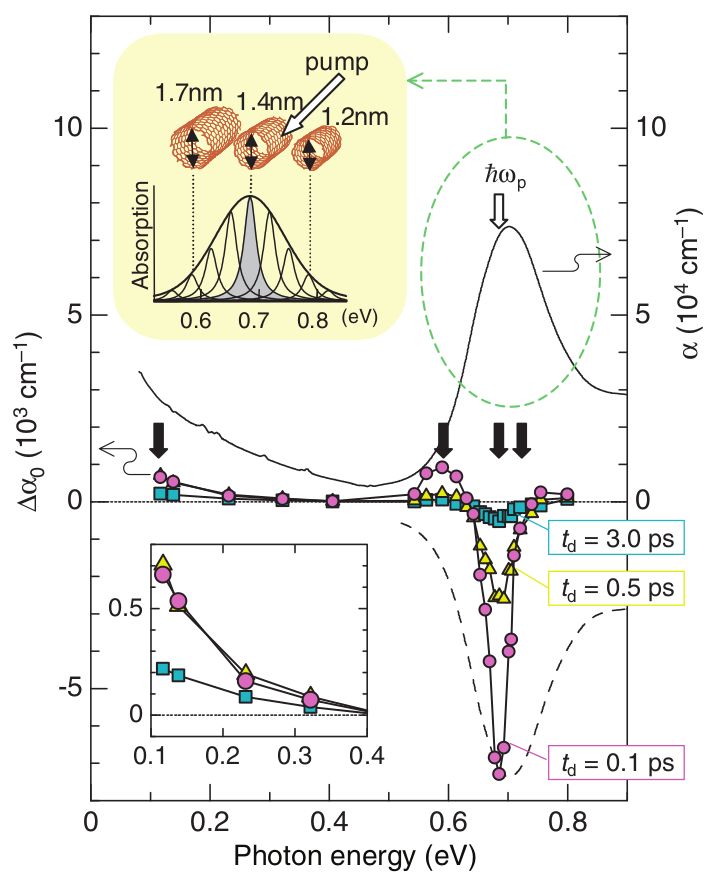
\includegraphics[scale=0.3]{images/chapter_prior_works/stark_shift_maeda}
	\caption{The top curve shows the absorption spectrum $\alpha$ of the SWCNT film studied by Maeda \textit{et al.} (2006) \cite{maeda2006gigantic}. Here, the absorption peak is inhomogenously broadened due to the presence of various nanotube chiralities within the film. The bottom traces show the change in absorption $\Delta \alpha_0$ as a function of time delay $t_\text{d}$ along with a plot of $-\alpha$ (dashed line). The lower inset figure shows a close-up of the left-hand region of the change in absorbance. The black arrows mark probe positions shown in Figure \ref{fig:dtt_2_maeda_2006}. Reproduced from Ref.\ \cite{maeda2006gigantic}.}
	\label{fig:abs_maeda_2006}
\end{figure}

Figure \ref{fig:dtt_2_maeda_2006} shows the dynamics probed at the labeled photon energies. Here, Maeda \textit{et al}.\ \cite{maeda2006gigantic} compute fits to the data using the phenomenological model
\begin{equation}
	\Delta \alpha_0(t_\text{d}) = A_1 \exp\left( \frac{-t_\text{d}^2}{\tau^2}\right) + \sum_\text{i=2,3} A_\text{i} \int^{t_\text{d}}_{-\infty} \mathrm{d} t^\prime \exp\left[ \frac{-(t_\text{d} - t^\prime)}{\tau_\text{i}} - \frac{t^{\prime 2}}{\tau^2}\right].
	\label{eq:fits_maeda_2006}
\end{equation}
The first term denotes the coherent, ultrafast component (UC) of the dynamics, which is expressed as a Gaussian function with width $\tau$ = 130 fs, the pulse duration of the optical pump. This term contains only a single fitting parameter $A_1$. The remaining two terms in the summation include two exponential decays associated with a fast decay component (FDC) and a slow decay component (SDC), respectively. These include the fitting parameters $A_\text{i}$ and $\tau_\text{i}$ (i = 2,3) for each component, respectively. For the data shown in Figure \ref{fig:dtt_2_maeda_2006}, they obtain the decay times 0.37 ps for the FDC ($\tau_2$) and 2 ps for the SDC ($\tau_3$).




\begin{figure}[H]
	\centering
	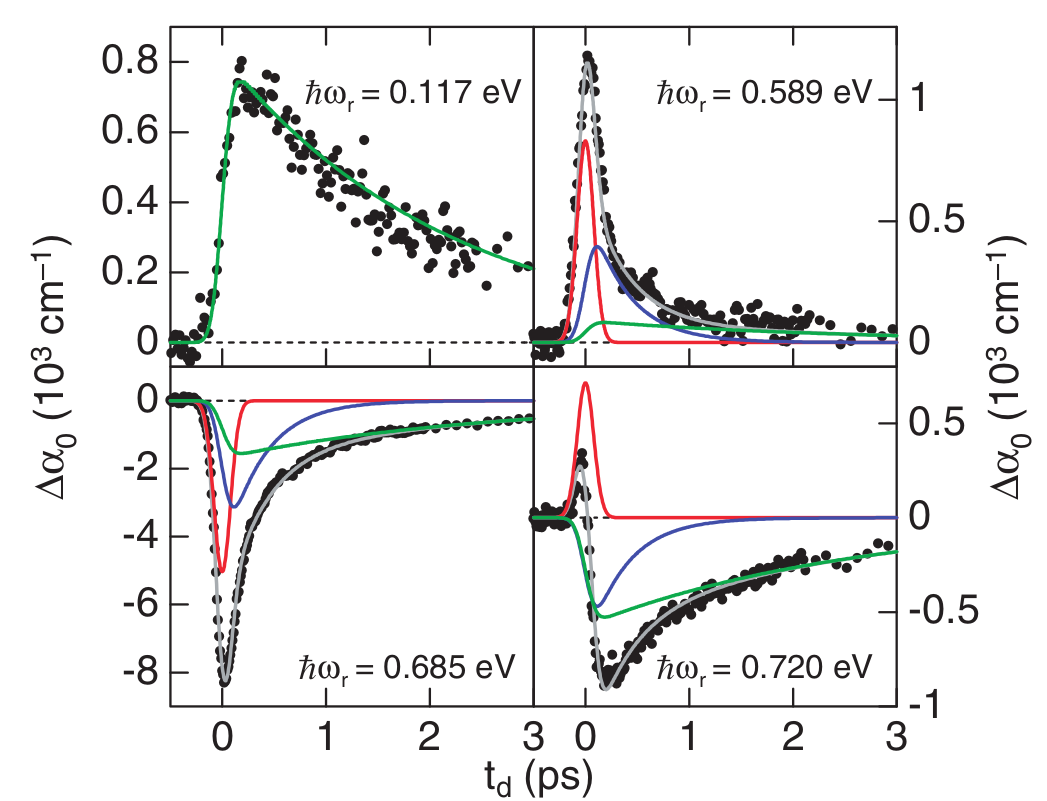
\includegraphics[scale=1.2]{images/chapter_prior_works/dtt_2_maeda_2006}
	\caption{Carrier dynamics probed at the indicated photon energy $\hbar \omega_\text{r}$ after the sample was photoexcited at 0.685 eV. The solid, grey lines indicate fits to the data using Equation \eqref{eq:fits_maeda_2006}. The red, blue, and green curves correspond to ultrafast, fast decay, and slow decay components, respectively. Reproduced from Ref.\ \cite{maeda2006gigantic}.}
	\label{fig:dtt_2_maeda_2006}
\end{figure}



\begin{figure}[H]
	\centering
	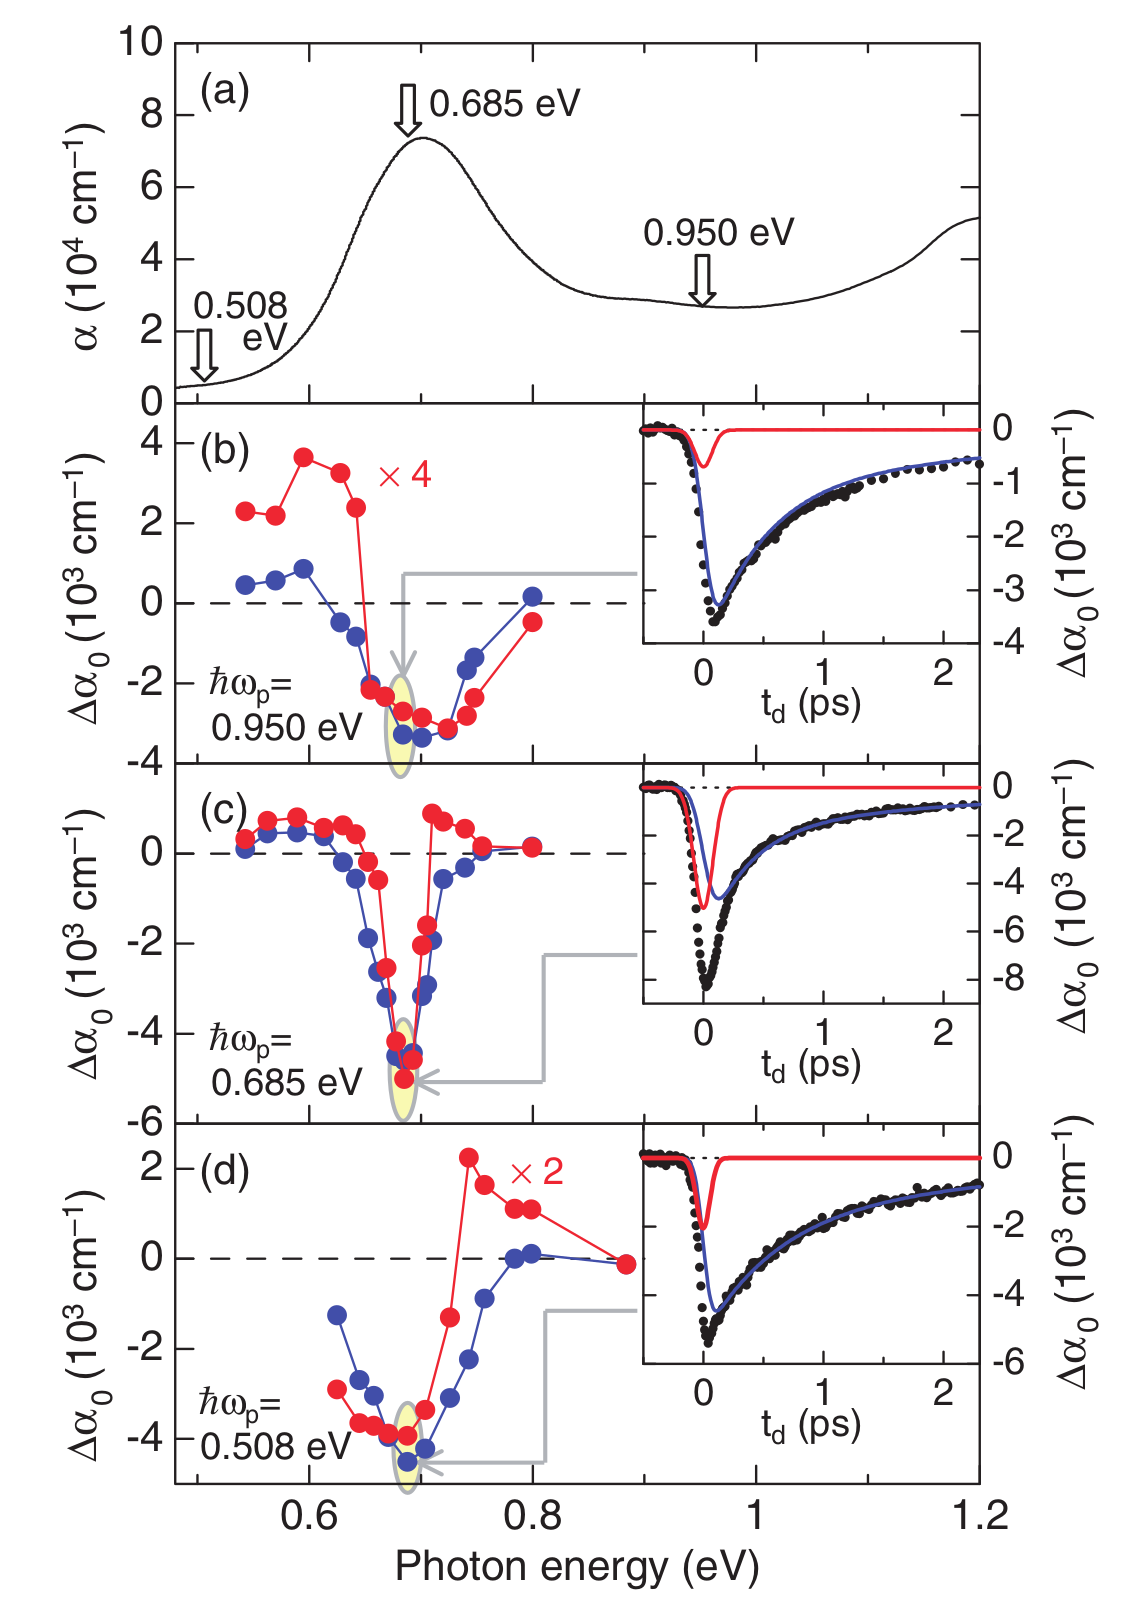
\includegraphics[scale=0.18]{images/chapter_prior_works/dtt_maeda_2006}
	\caption{(a) Absorption spectrum $\alpha$ of the SWCNT film studied by Maeda \textit{et al}. \cite{maeda2006gigantic}. The arrows mark pump energies $\hbar \omega_\text{p}$ used to obtain the results shown in the figures below. (b)-(e) Change in the absorption spectrum after the sample was photoexcited at (b) 0.950, (c) 0.685 and (d) 0.508 eV. The red circles correspond to maximum change in the absorption due to the ultrafast component $A_1$ after fitting the data to Equation \eqref{eq:fits_maeda_2006}. Similarly, the blue circles show the change in absorption associated with the sum of the fast and slow decay components $A_2 + A_3$. The inset figures show the dynamics probed at 0.685 eV in each scenario as well as fits to the data which correpond to the ultrafast component (red) and the sum of the fast and slow decay components (blue). Reproduced from Ref.\ \cite{maeda2006gigantic}.}
	\label{fig:dtt_maeda_2006}
\end{figure}


The observed dynamics certainly changed when the sample was photoexcited at other photon energies. Figure \ref{fig:dtt_maeda_2006} presents these results. When photoexciting the sample above the $E_{11}$ resonance, the ultrafast component (UC) measured at each probe photon energy suggested that a redshift of the $E_{11}$ occured. Photoexcitations below the $E_{11}$ transition instead caused a \textit{blueshift} of the $E_{11}$ peak.

These results certainly agree with those predicted by Equation \eqref{eq:ose_blueshift} as pumping the sample above and below the resonance corresponds to positive and negative detunings, respectively. However, when the photon energy of the optical pump equaled that of the $E_{11}$ transition, the spectral shape of the ultrafast component suggested that optical pump coherently splits the $E_{11}$ resonance into two states. This phenomenon is also consistent with the optical Stark effect occuring within a two-level system.

Matsumoto \textit{et al}.\ (2006) \cite{matsumoto2006optical} observed the optical Stark effect in a CoMoCAT SWCNT film sample. Here, each nanotube was individually suspended using carboxymethylcellose (CMC), a transparent polymer \cite{matsumoto2006optical}. Figure \ref{fig:abs_dtt_matsumoto} shows a key result of their work. Here, the (6,5) $E_{11}$ resonance located at 1.25 eV is inhomogenously broadened due to the nearby $E_{11}$ resonances of (7,5) and (8,3) nanotubes in the sample. Furthermore, when the sample was photoexcited below the $E_{11}$ transition at a photon energy of 1.14 eV with a fluence of \SI{34}{\micro \joule / \cm\squared}, the differential transmission suggested that the $E_{11}$ state coherently blueshifted at 0 ps.

This blueshift immediately disappeared at 0.3 ps. Hence, the signals observed at 0.3 and 10 ps corresponded to the relaxation of real carriers created via multiphoton processes. Figure \ref{fig:dtt_matsumoto} shows that the data measured at 0 ps is linearly proportional to the first derivative of the absorption spectrum, which agrees with the observations made by Song \textit{et al} \cite{song2006optical}. From this, they deduced that the optical pump produced a blueshift of $1.1 \pm 0.3$ meV.

\begin{figure}[H]
	\centering
	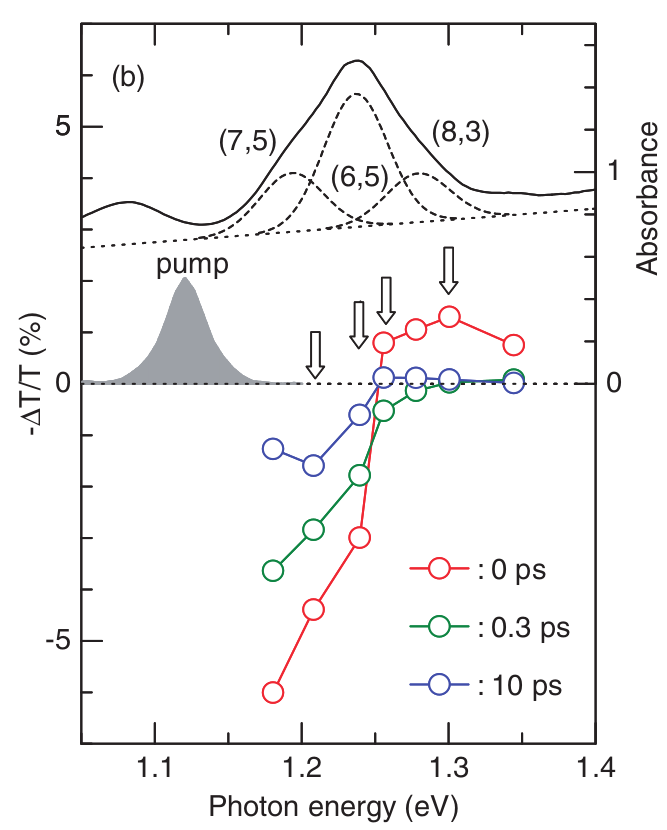
\includegraphics[scale=1.25]{images/chapter_prior_works/abs_dtt_matsumoto}
	\caption{The top curve shows the absorbance spectrum of the CoMoCAT suspension studied by Matsumoto \textit{et al}.\ (2006) \cite{matsumoto2006optical}. The resonance located at 1.25 eV corresponds to the $E_{11}$ transition of (6,5) nanotubes. It is inhomogenously broadened due to a small population of (7,5) and (8,3) nanotubes that have their own $E_{11}$ resonances nearby. The bottom traces show differential transmision spectra at the indicated time delays after the sample was photoexcited at 1.14 eV at a fluence of \SI{34}{\micro \joule / \cm\squared}. Finally, the shaded figure represents the spectrum of the optical pump. Reproduced from Ref.\ \cite{matsumoto2006optical}.}
	\label{fig:abs_dtt_matsumoto}
\end{figure}


\begin{figure}[ht]
	\centering
	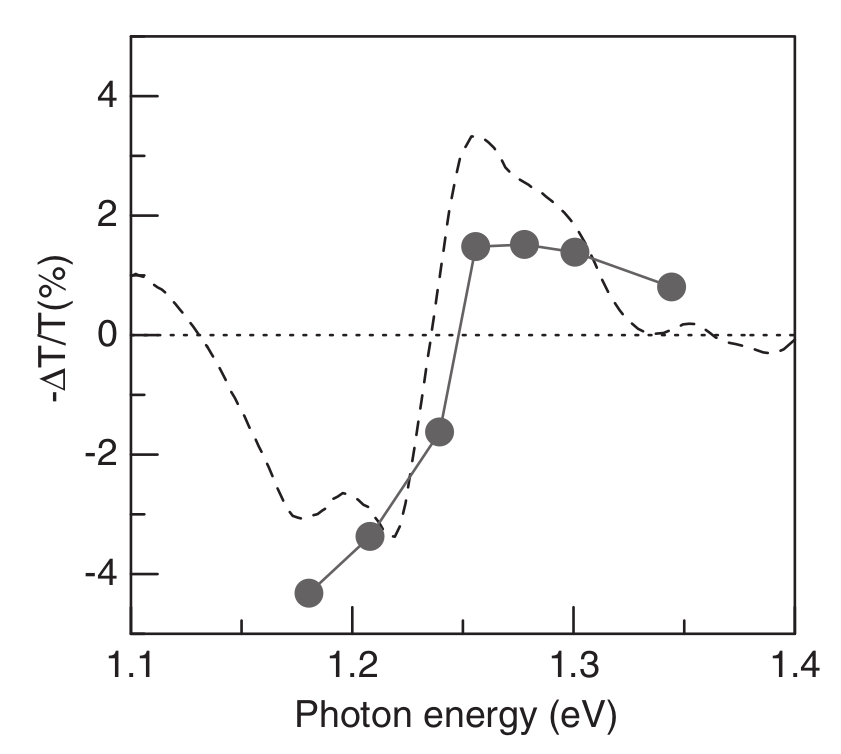
\includegraphics[scale=0.3]{images/chapter_prior_works/dtt_matsumoto}
	\caption{The plot shows the differential transmission measured at 0 ps from Figure \ref{fig:abs_dtt_matsumoto}. The dashed curve corresponds to the first derivative of the absorbance spectrum $\partial \alpha / \partial \omega$. Using this data, Matsumoto \textit{et al}.\ \cite{matsumoto2006optical} estimated that the $E_{11}$ resonance coherently shifted by $1.1 \pm 0.3$ meV. Reproduced from Ref.\ \cite{matsumoto2006optical}.}
	\label{fig:dtt_matsumoto}
\end{figure}

Tao \textit{et al}.\ (2009) \cite{tao2009subpicosecond} also demonstrated how the detuning of the optical pump affects the optical Stark effect. In this work, they studied a film of CoMoCAT SWCNTs created by individually suspending the nanotubes using sodium cholate hydrate in an aqeuous solution. This suspension was then mixed in a gelatin to create a homogenous thin film suitable for optical measurements. Tao \textit{et al}.\ (2009) \cite{tao2009subpicosecond} carried out experiments where the sample was photoexcited at photon energies below and above the (6,5) $E_{11}$ resonance energy.

Figure \ref{fig:detuning_tao_2009} shows how the energy shift $\Delta E_\text{S}$ and broadening $\Delta E_\text{B}$ of the $E_{11}$ transition scales with the detuning $E_\text{d}$ of the optical pump. Here, they observed that $\Delta E_\text{S}$ scales linearly with $E_\text{d}^{-1}$ as predicted by Equation \eqref{eq:ose_blueshift}. The $E_{11}$ peak also appears to broaden in these scenarios, which they attributed to scattering events between virtual and real excitons.

\begin{figure}[ht]
	\centering
	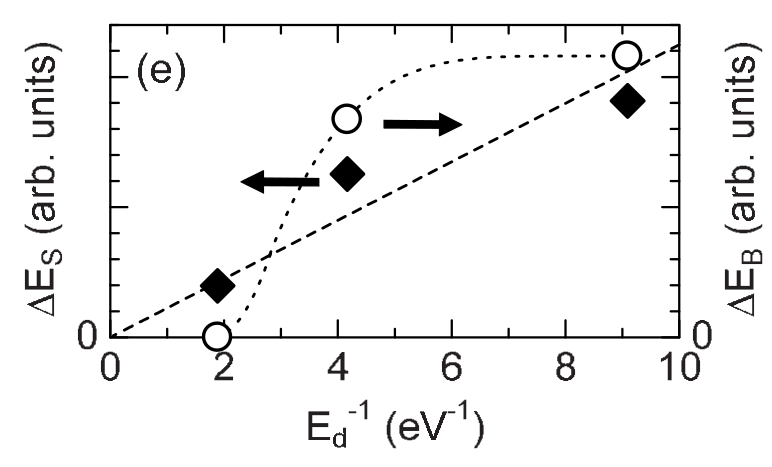
\includegraphics[scale=0.35]{images/chapter_prior_works/fluence_tao_2009}
	\caption{Experimental data reported by Tao \textit{et al}.\ (2009) \cite{tao2009subpicosecond}. The plot shows how the coherent shift $\Delta E_\text{S}$ as well as the broadening $\Delta E_\text{B}$ of the $E_{11}$ resonance changed with the detuning $E_\text{d}$ of the optical pump. Here, $\Delta E_\text{S}$ scales linearly with $E_\text{d}^{-1}$ as predicted by Equation \eqref{eq:ose_blueshift}. Reproduced from Ref.\ \cite{tao2009subpicosecond}.}
	\label{fig:detuning_tao_2009}
\end{figure}

Figure \ref{fig:abs_dtt_tao_2009} shows how the creation of real carriers can mask the presence of the optical Stark effect. When exciting the sample at or below the $E_{11}$ resonance energy, a coherent blueshift of the $E_{11}$ resonance occurred at a time delay of 0 ps and immediately disappeared at 0.3 ps. This coherent component was easily isolated as shown by the shaded regions of the right-hand plots. However, when the sample was photoexcited above the $E_{11}$ resonance, a coherent shift was not easily resolved and the dynamics were instead dominated by the relaxation of real carriers.

\begin{figure}[ht]
	\centering
	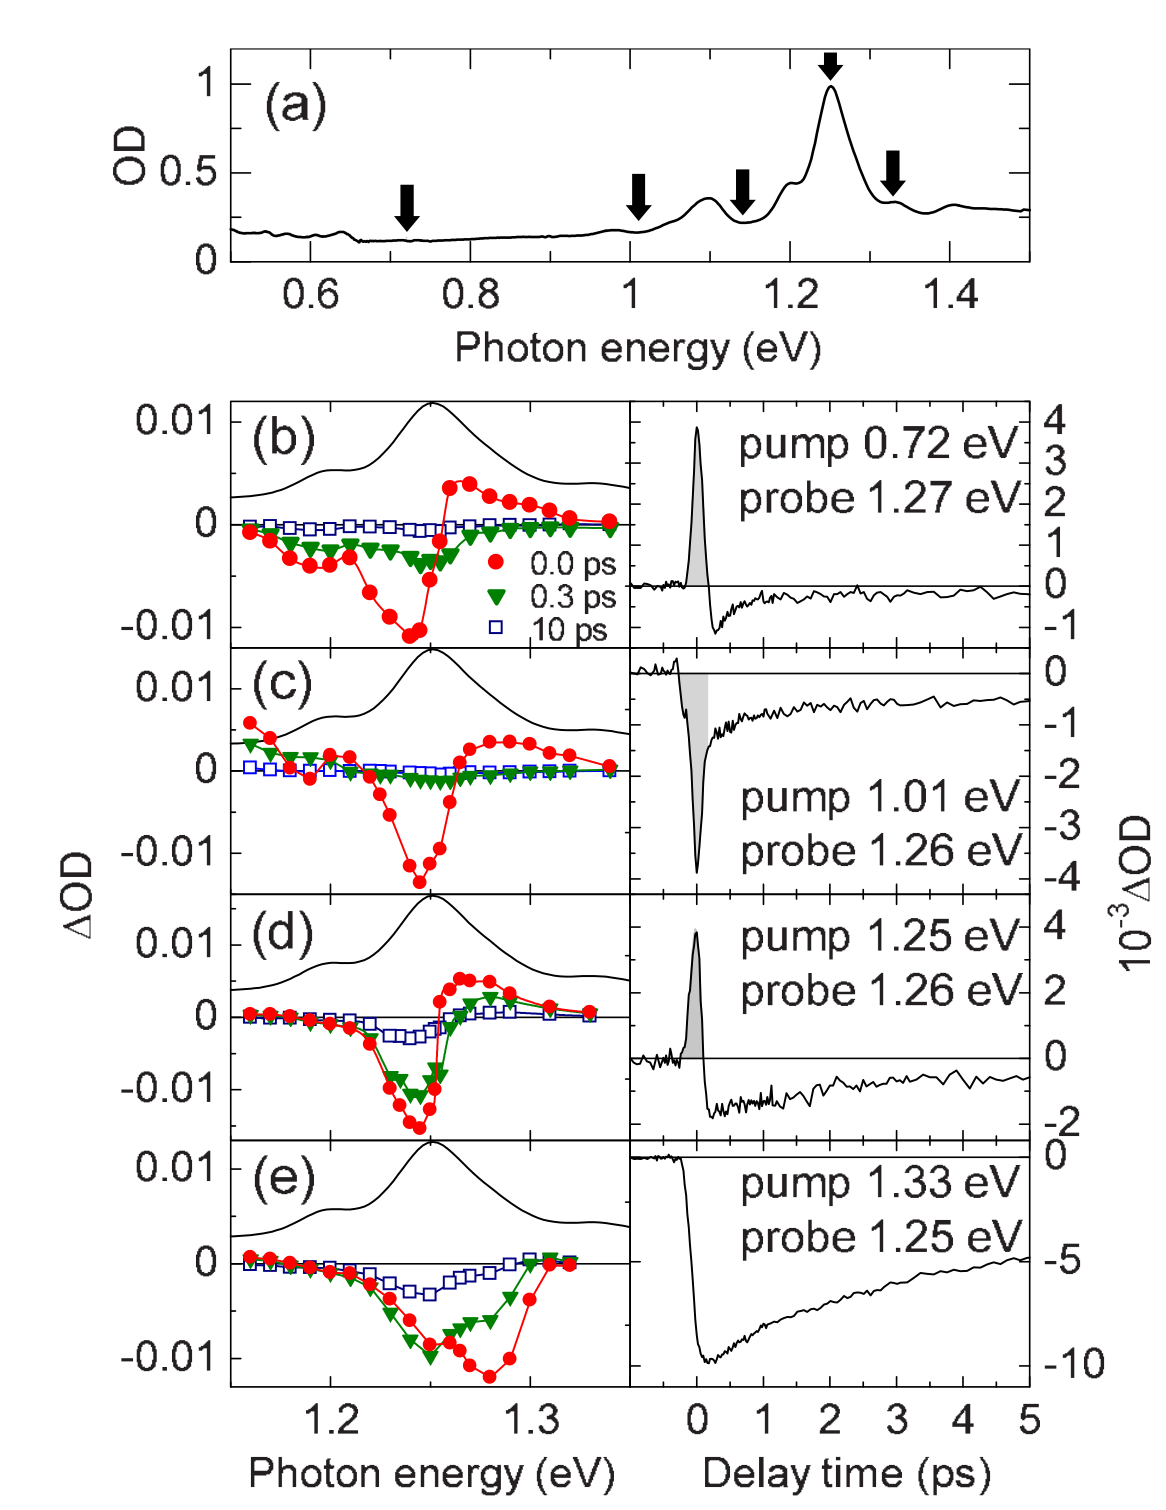
\includegraphics[scale=0.25]{images/chapter_prior_works/abs_dtt_tao_2009}
	\caption{(a) The absorption spectrum for the CoMoCAT SWCNT film sample studied by Tao \textit{et al} (2009) \cite{tao2009subpicosecond}. The peak at 1.25 eV corresponds to the (6,5) $E_{11}$ resonance. It is inhomogenously broadened by the $E_{11}$ resonances of (7,5) and (8,3) nanotubes. The black arrows indicate photon energies of the optical pump for the pump probe measurements in the bottom figures. (b) - (e) Optical responses measured after photoexciting at (b) 0.72 eV, (c) 1.01 eV, (d) 1.25 eV, and (e) 1.33 eV.  Reproduced from Ref.\ \cite{tao2009subpicosecond}.}
	\label{fig:abs_dtt_tao_2009}
\end{figure}

In summary, the literature regarding the optical Stark Effect observed in SWCNTs is quite consistent unlike those describing the effects of exciton-exciton annihilation. In each study, a coherent blueshift of the $E_{11}$ resonance was observed and well described by Equation \eqref{eq:ose_blueshift}. A key limitation here is that creation of real carriers can easily obfuscate optically-induced coherent shifts of the $E_{11}$ transition. Nonetheless, the fact that carriers relax on picosecond timescales mitigates this to some extent and renders SWCNTs suitable for ultrafast all-optical switching applications.
%\section{Discussion}


%Conflicting reports of exciton-exciton annihilation. Consensus regarding efficiency of exciton exciton isn't so clear. There could be a number of reasons for disagreements in each work. These can include, type of sample studied, power density of the optical pump as well as pump wavelength. Samples in early studies used HiPco or CoMoCAT dispersions which contained several different chiralities. As noted by Ostojic \textit{et al}.\ (2004), optical excitations can cause both resonant and non-resonant excitations in the ensemble. Moreover, multi-photon processes occuring in metallic nanotubes, which have resonances at higher photon energies, could also play a role.

%Exciton sizes can vary depending on dielectric environment \cite{mann201613}.

%One question: Do carrier relaxation processes differ when exciting resonantly or nonresonantly? If so, how?

%Does phonon side-band play a role here? It has been ignored in early studies as $E_{11}$ and $E_{22}$ resonance are dominant in optical absorption spectrum.
%Wang \textit{et al} (2004) pumped at 810 nm which is right between $E_{11}$ and $E_{22}$ of many of the semiconducting in their sample.

%Dielectric environment can have an effect on
